\chapter{Experimental results}
\label{experiments}
In this chapter we compare the performance of IDA* and various versions of MCTS on Samegame and Sokoban.

\section{Samegame}
As a preliminary part of our study, we replicated the experiment performed by Schadd et al. \cite{DBLP:journals/kbs/SchaddWTU12} and compared our results. We ran an experiment using our implementation of SP-MCTS. Due to differences of the Samegame implementation, our program was considerably slower than the one used in \cite{DBLP:journals/kbs/SchaddWTU12}. Our implementation performed an average of 2630 iterations per second against the 13888 iterations per second obtained by \cite{DBLP:journals/kbs/SchaddWTU12}. The program used in \cite{DBLP:journals/kbs/SchaddWTU12} performed 100000 iterations and 1000 restarts with search time distributed per move, which --- considering an average solution length of 64.4 --- resulted in an average of 1553 iterations per move. We decided to keep execution time as a constraint instead of number of iterations, and to achieve that, we reduced the number of randomized restarts from 1000 to 180. The resulting MCTS configuration used a UCT constant of 4.31, a SP-MCTS constant of 96.67, 1500 iterations per move and 180 restarts. As a result, we obtained a score of 73586 in the standard test set \cite{highscore}. Table \ref{tab:samegame_spmctsresults} shows the results for each level in the test set in comparison with the results obtained by \cite{DBLP:journals/kbs/SchaddWTU12} and HGSTS \cite{Edelkamph}, the top scoring documented algorithm for Samegame.
\begin{table}[!h]
    \centering
    \begin{tabular}{ l | l | l | l }
          \# & Our SP-MCTS & SP-MCTS(3) & HGSTS \\
          \hline			
          1 & 2671 & 2919 & 2561 \\
          2 & 3723 & 3797 & 4995 \\
          3 & 3051 & 3243 & 2858 \\
          4 & 3781 & 3687 & 4051 \\
          5 & 4001 & 4067 & 4633 \\
          6 & 4189 & 4269 & 5003 \\
          7 & 2359 & 2949 & 2717 \\
          8 & 3881 & 4043 & 4622 \\
          9 & 4723 & 4769 & 6086 \\
          10 & 2623 & 3245 & 3628 \\
          11 & 2689 & 3259 & 2796 \\
          12 & 3083 & 3245 & 3710 \\
          13 & 2881 & 3211 & 3271 \\
          14 & 2687 & 2937 & 2432 \\
          15 & 3021 & 3343 & 3877 \\
          16 & 4915 & 5117 & 6074 \\
          17 & 4717 & 4959 & 5166 \\
          18 & 5109 & 5151 & 6044 \\
          19 & 4843 & 4803 & 5019 \\
          20 & 4639 & 4999 & 5175 \\
          \hline  
          Total & 73586 & 78012 & 84718 \\
          \hline 
    \end{tabular}
    \caption[Our SP-MCTS results]{Results of our implementation of SP-MCTS}
    \label{tab:samegame_spmctsresults}
\end{table}

\medskip\noindent
Our results are overall worse than the ones obtained by the original authors, but considering the difference in the number of restarts, such outcome is in line with what we expected. This experiment allowed us to ensure that our implementation is coherent to \cite{DBLP:journals/kbs/SchaddWTU12} and to proceed with further experiments with a baseline for performance comparisons.

\subsection{Node Elimination \& Cycles Avoidance}
We started our optimizations analysis with Node Elimination. To reduce computation time we performed the tests with 1500 iterations without randomized restarts. The baseline was obtained with SP-MCTS and no other optimization. We then enabled Node Elimination and compared the results, shown in Table \ref{tab:samegame_nodeelimination}.
\begin{table}[!h]
    \centering
    \begin{tabular}{l|l}
        Configuration & Score\\
        \hline
        Baseline & 57965 \\
        Node Elimination & 56940
    \end{tabular}
    \caption{Node Elimination outcome}
    \label{tab:samegame_nodeelimination}
\end{table}
Node Elimination obtained a score lower than the baseline. We can assume this is due to the fact that in Samegame revisiting terminal nodes can help in the estimation of the action value function.

\medskip\noindent
Since in Samegame cycles can't occur, there was no need to test Cycles Avoidance.

\subsection{Parameters tuning}
In order to take full advantage of the optimizations we described in Section \ref{proposedsolution}, we needed to tune their parameters to obtain the best configuration. In particular, we executed repeated searches with different values for the RAVE threshold and the memory budget of Node Recycling. We also tuned again the UCT constant with UCB1-Tuned, since \cite{DBLP:journals/kbs/SchaddWTU12} performed the tuning with the SP-MCTS formula. Node Elimination has no parameters so it didn't require tuning. As before we performed the tests with 1500 iteration and no randomized restarts. The results of the tuning process are shown in Tables \ref{tab:samegame_tuningrave} and \ref{tab:tuningrecycling}.
\begin{table}[!h]
    \centering
    \begin{tabular}{l|l}
        V & Score \\
        \hline 
        1 & 57965 \\
        5 & 46663 \\
        10 & 47722 \\
        15 & 49519 \\
        25 & 49239 \\
        50 & 52028 \\
        100 & 54738 \\
    \end{tabular}
    \caption[RAVE thresholds scores]{Scores obtained with different RAVE thresholds. The first row is equivalent to disabling RAVE and represents our baseline.}
    \label{tab:samegame_tuningrave}
\end{table}

\medskip\noindent
 If we only consider the results with RAVE enabled, it reached the highest score with $V=100$, but contrary to our expectations, it had an overall negative impact on the score. We concluded that the assumption upon which RAVE is based, does not hold for Samegame, i.e. moves performed later on in a simulation can't be considered as if they were performed at the beginning.

\begin{table}[!h]
    \centering
    \begin{tabular}{l|l}
        Nodes & Score \\
        \hline 
        300 & 55302 \\
        600 & 57798 \\
        900 & 54601 \\
        1200 & 56532 \\
        1500 & 57965 \\
    \end{tabular}
    \caption[Node Recycling memory budgets scores]{Scores obtained with Node Recycling and different memory budgets. The last row is equivalent to disabling Node Recycling and represents our baseline.}
    \label{tab:tuningrecycling}
\end{table}

\medskip\noindent
Node Recycling reduced the score too, although less than RAVE, which means that it may prune good sub-trees in Samegame. With a memory budget of $600$ nodes it produced a score close to the baseline.

%figures \ref{fig:samegametuning} and \ref{fig:samegameucb1tuning}. 

%\begin{figure}[!h]
%\centering
%\subfigure[Scores obtained with different RAVE thresholds]{
%\label{fig:samegame_tuningrave}
%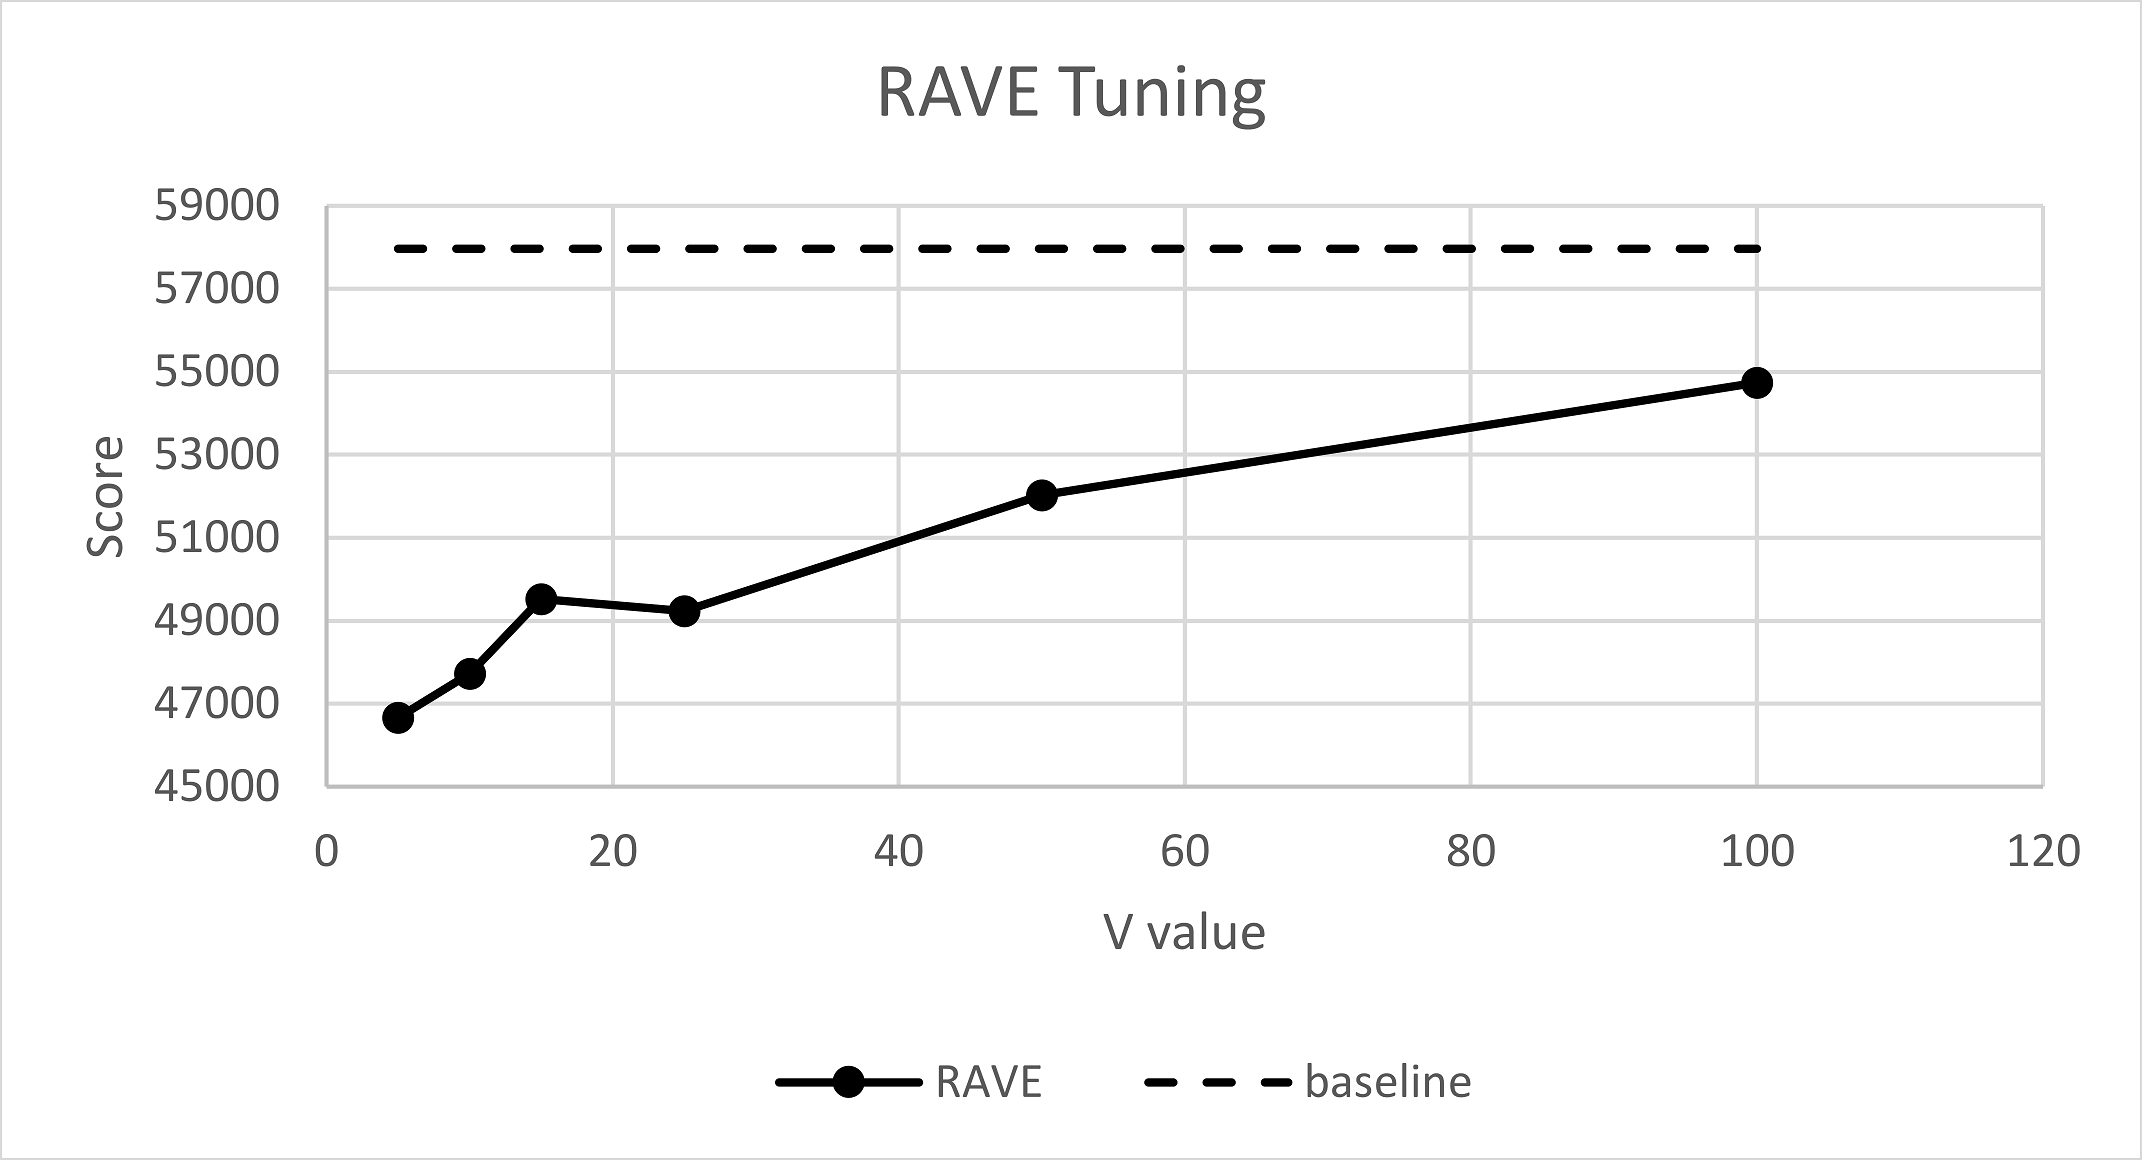
\includegraphics[width=0.8\linewidth]{pictures/SamegameRaveTuning.png}}
%\subfigure[Scores obtained with different memory budgets]{
%\label{fig:samegame_tuningrecycling}
%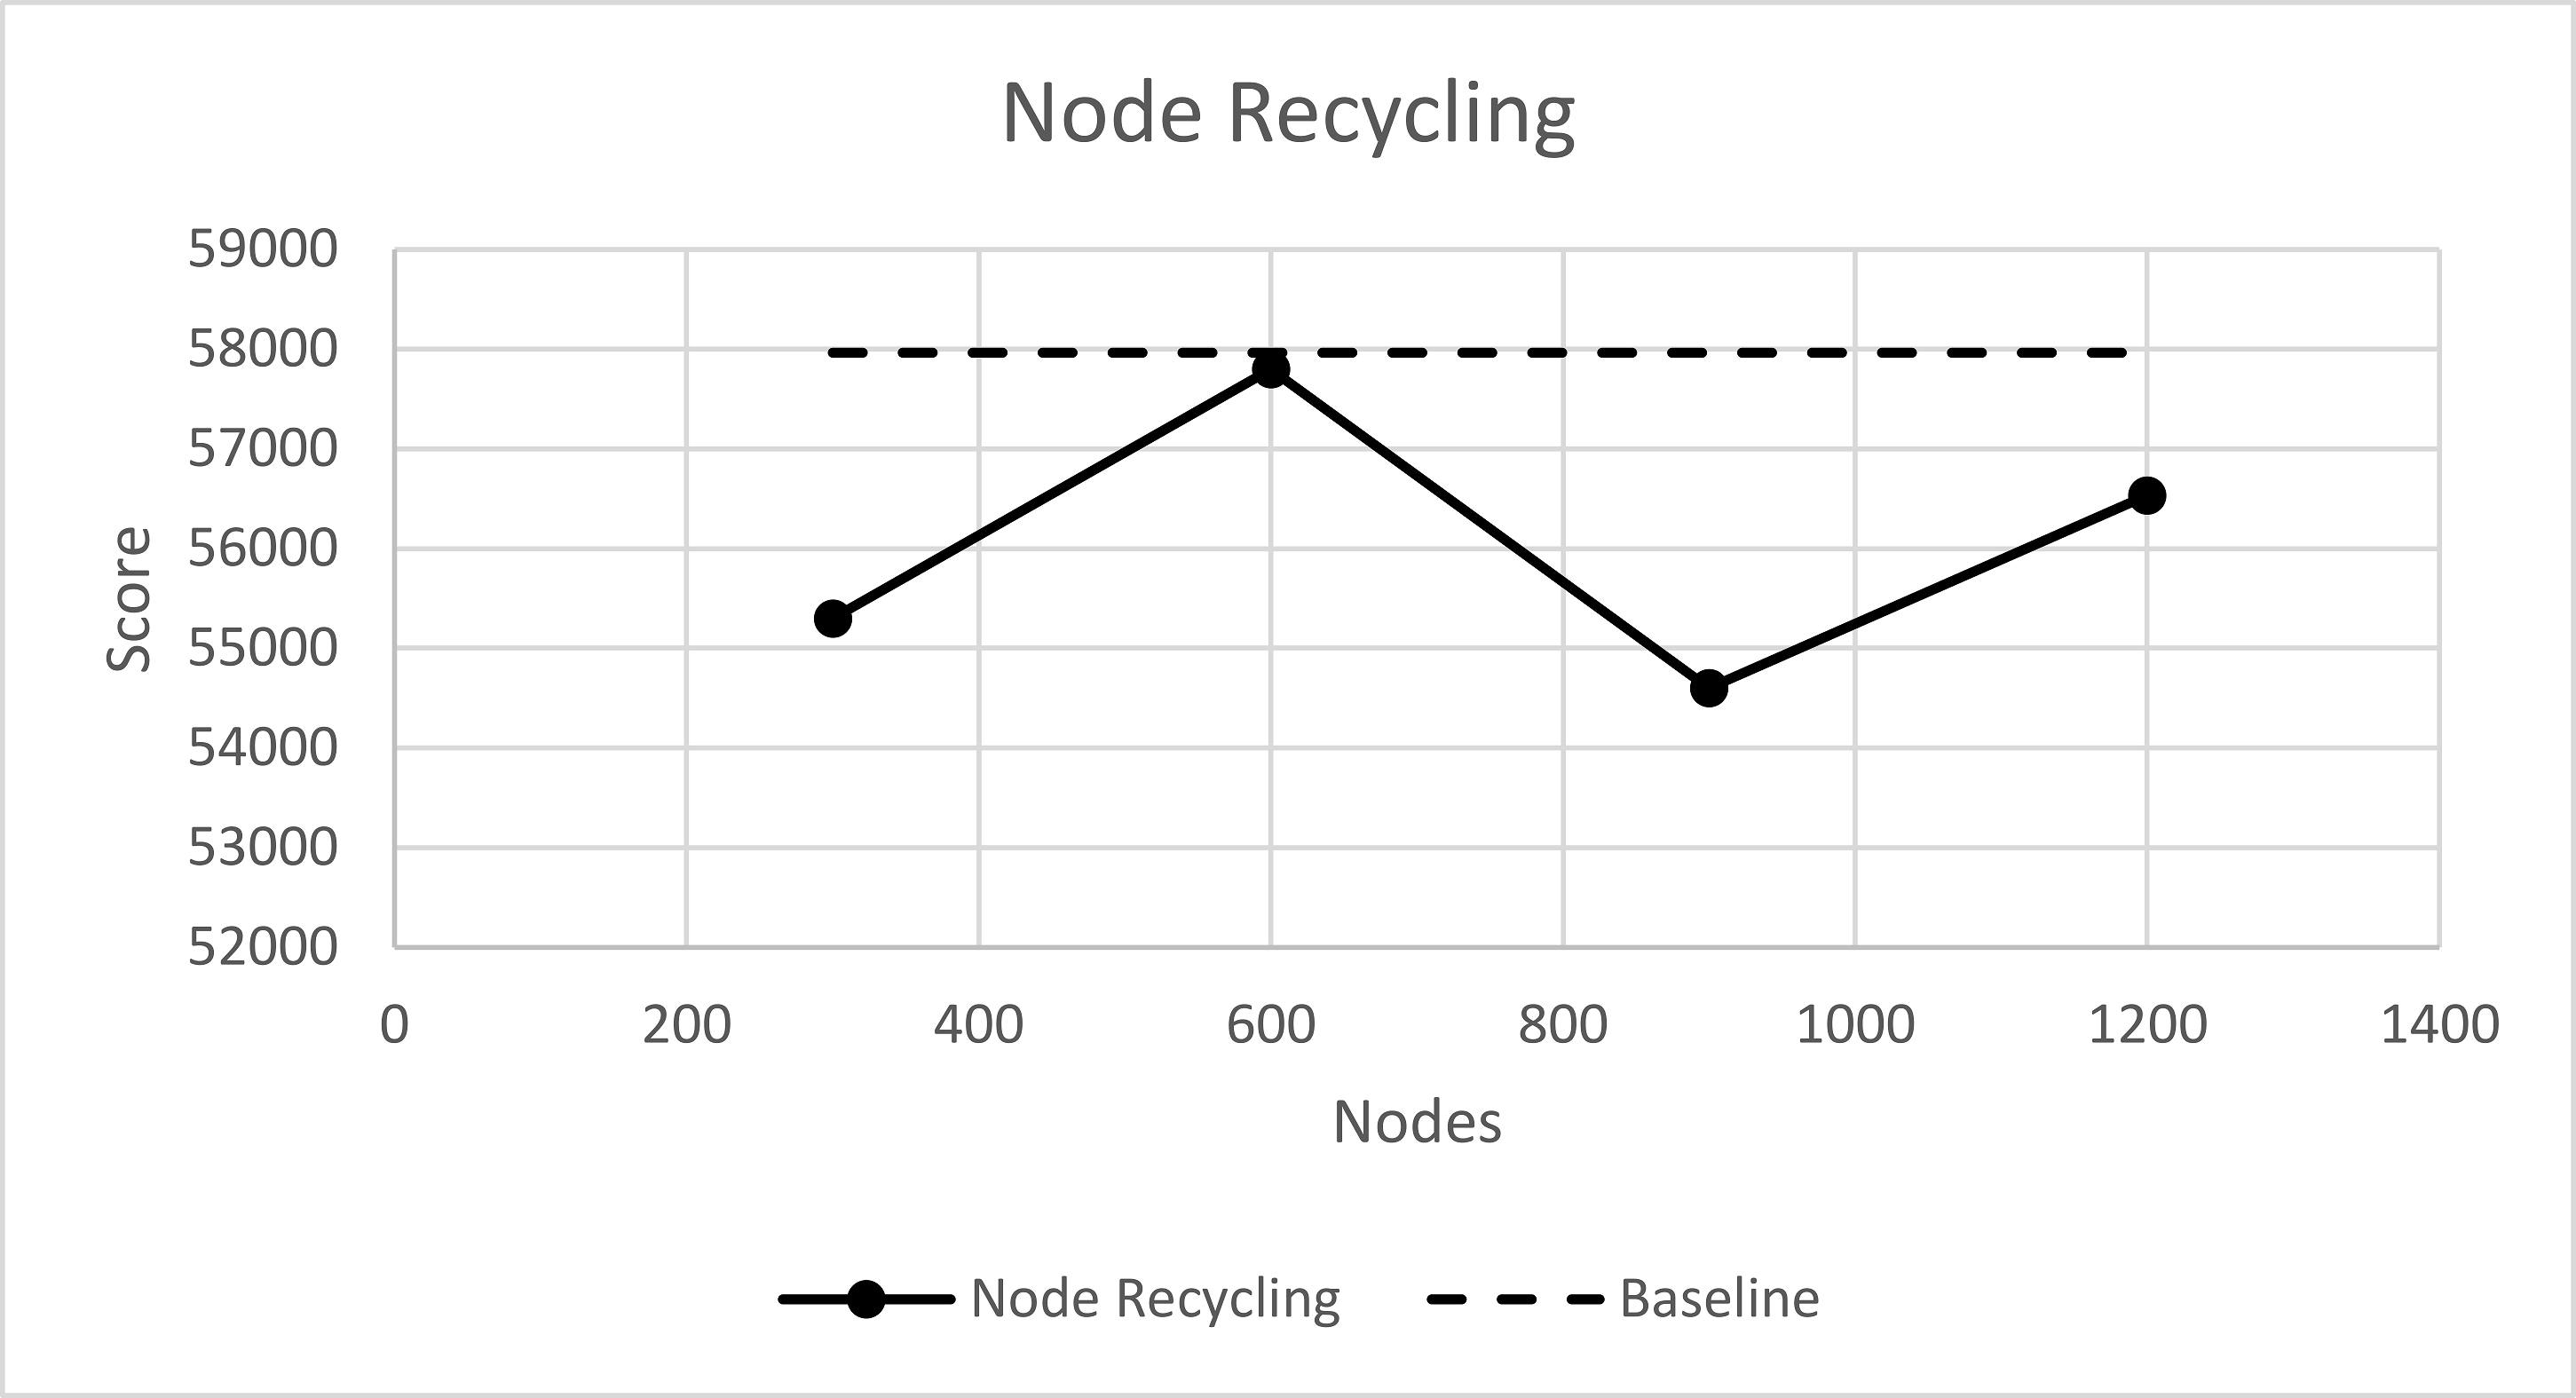
\includegraphics[width=0.8\linewidth]{pictures/SamegameNodeRecyclingTuning.png}}
%\caption{Samegame Tuning}
%\label{fig:samegametuning}
%\end{figure}

\medskip\noindent
As shown in Figure \ref{fig:samegameucb1tuning}, UCB1-Tuned performed better than SP-MCTS with different values but reached the highest score with a constant value of 10.

\begin{figure}[!h]
    \centering
    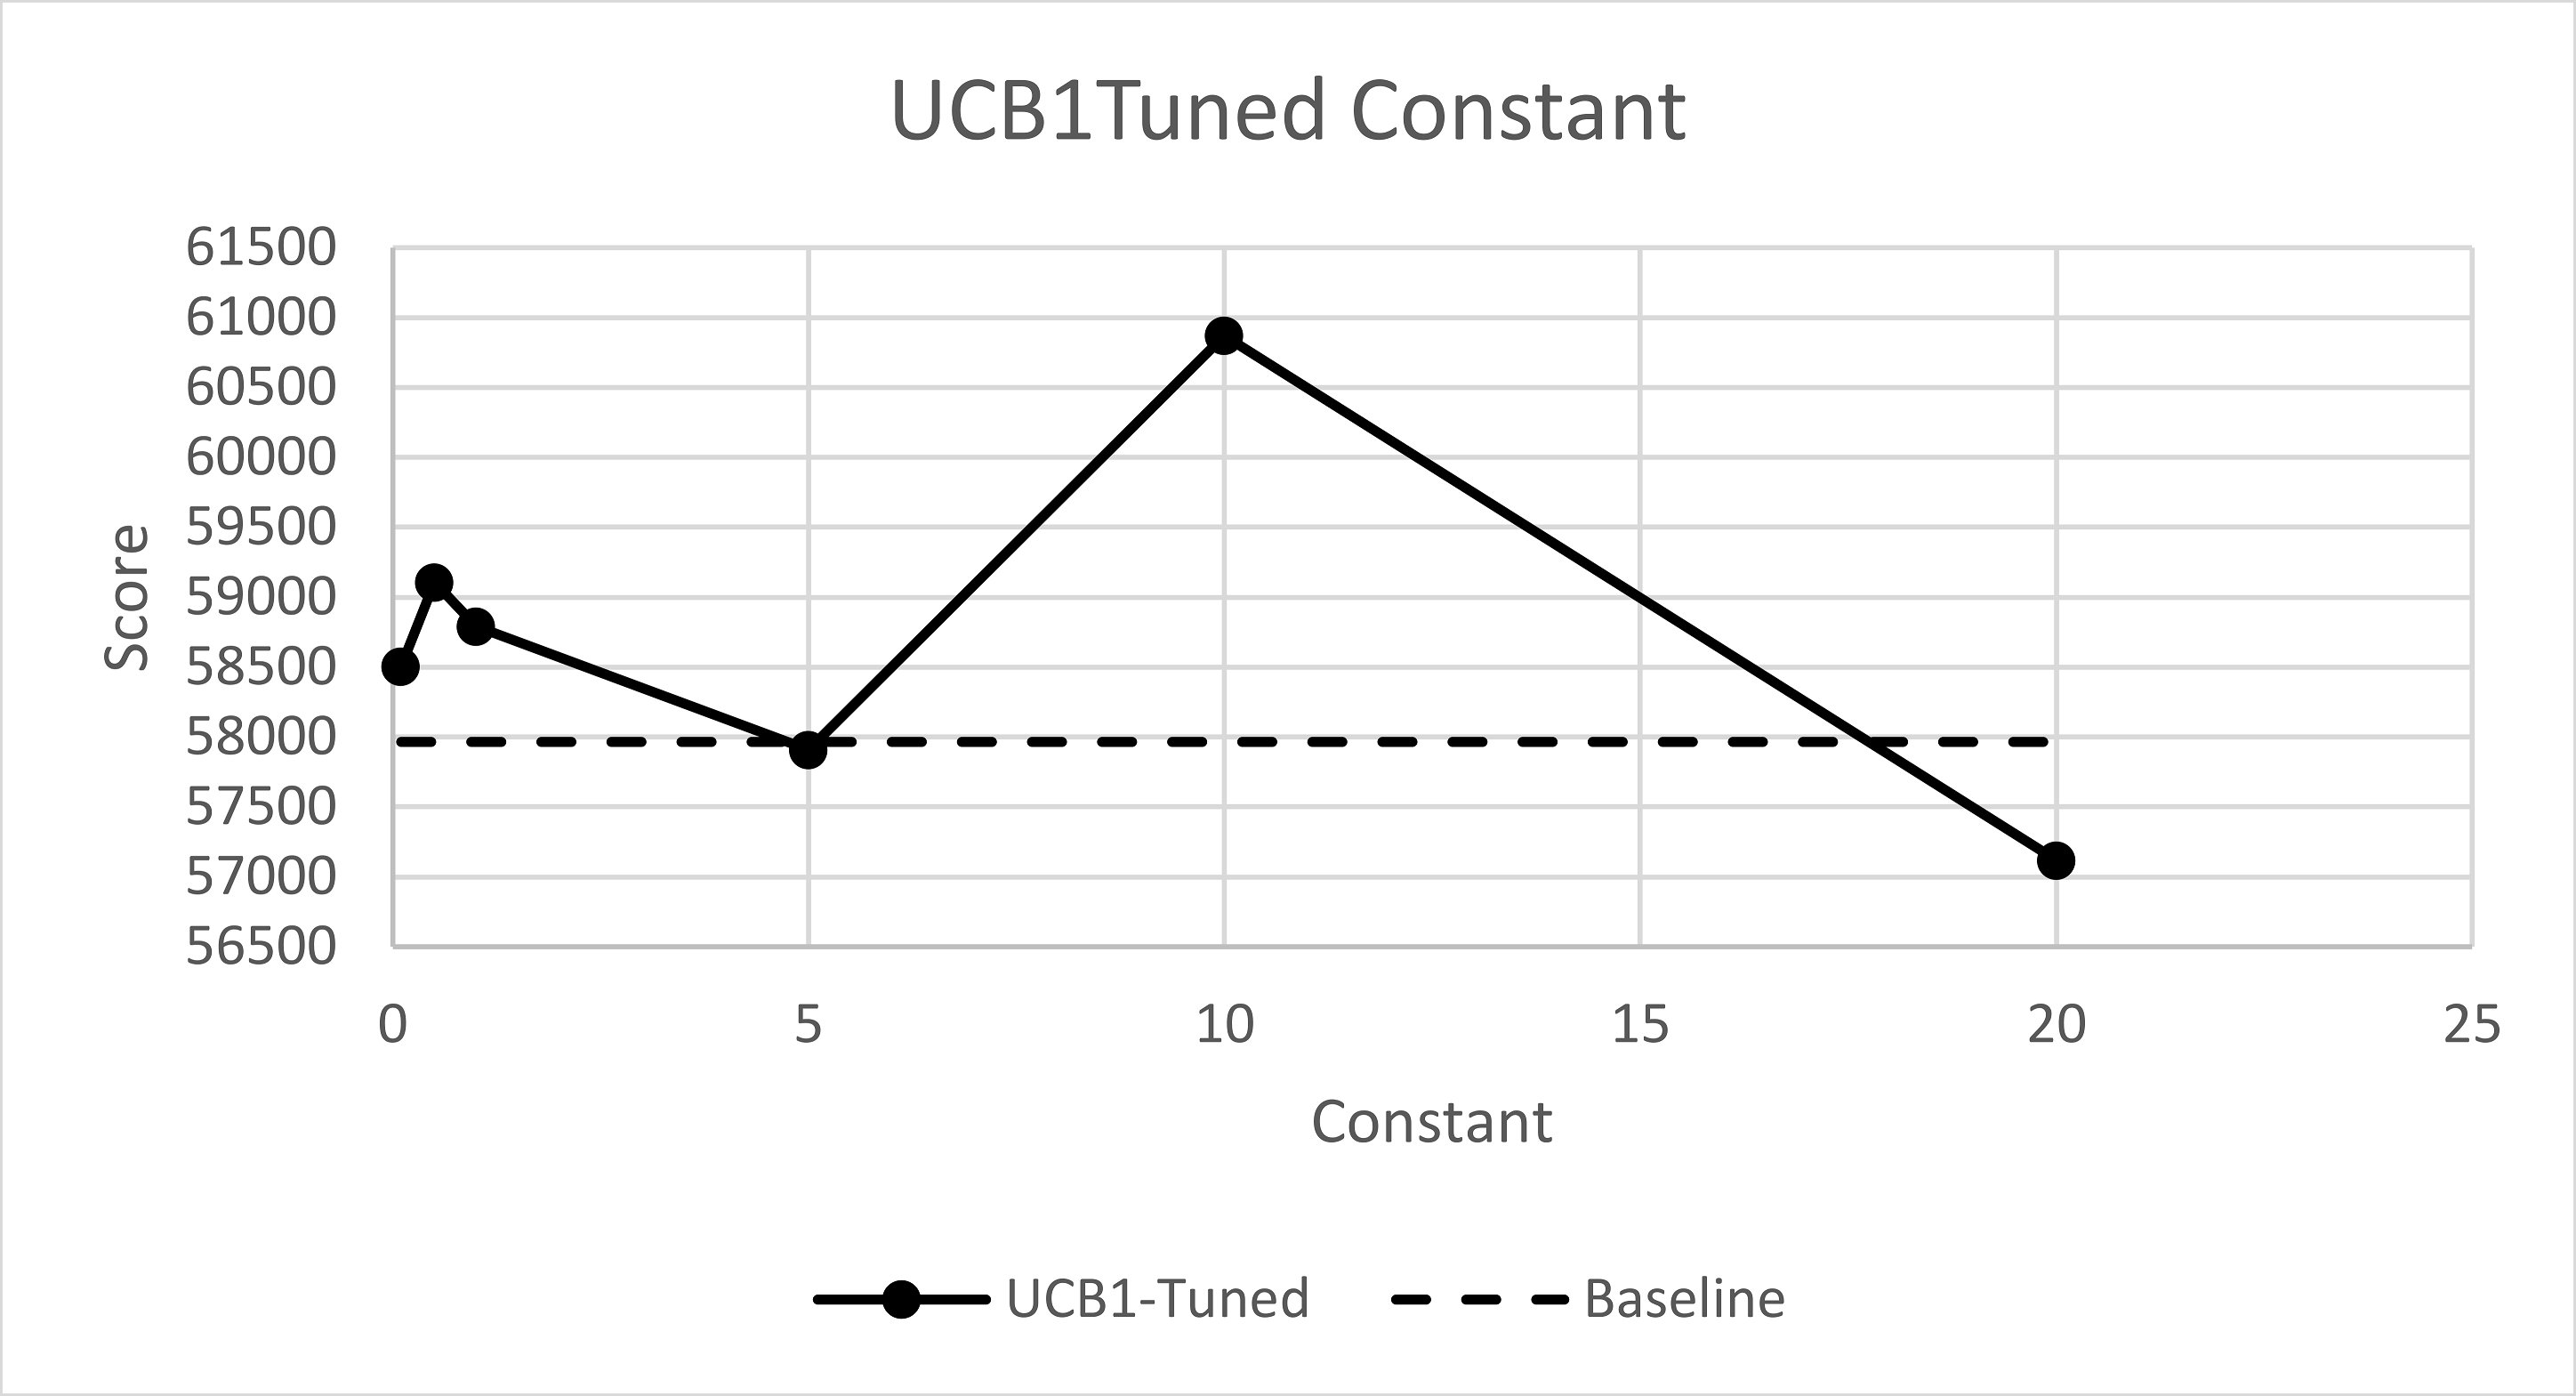
\includegraphics[width=0.8\linewidth]{pictures/SamegameUCB1Tuned.png}
    \caption[UCB1-Tuned constants scores]{Scores obtained with different constant values}
    \label{fig:samegameucb1tuning}
\end{figure}

\subsection{Results}
Considering the results obtained in previous experiments, we performed a comparison between our basic version of SP-MCTS and SP-MCTS with UCB1-Tuned. For this evaluation we used 1500 iterations and 180 restarts. The results of this comparison can be seen in Table \ref{tab:samegame_optresults}. UCB1-Tuned obtained a score of 74136, surpassing our previous score by 550 points.

\begin{table}[!h]
    \centering
    \begin{tabular}{ l | l | l }
          \# & Our SP-MCTS & UCB1-Tuned \\
          \hline			
          1 & 2671 & 2615 \\
          2 & 3723 & 3763\\
          3 & 3051 & 3251\\
          4 & 3781 & 3607\\
          5 & 4001 & 3891\\
          6 & 4189 & 4147\\
          7 & 2359 & 2675\\
          8 & 3881 & 3875\\
          9 & 4723 & 4689\\
          10 & 2623 & 2601\\
          11 & 2689 & 2683\\
          12 & 3083 & 3125\\
          13 & 2881 & 2805\\
          14 & 2687 & 2687\\
          15 & 3021 & 3329\\
          16 & 4915 & 4891\\
          17 & 4717 & 4639\\
          18 & 5109 & 5117\\
          19 & 4843 & 4869\\
          20 & 4639 & 4877\\
          \hline  
          Total & 73586 & 74136\\
          \hline 
    \end{tabular}
    \caption[SP-MCTS versus UCB1-Tuned in Samegame]{Comparison between results obtained by our SP-MCTS implementation and UCB1-Tuned enhancement.}
    \label{tab:samegame_optresults}
\end{table}

\medskip\noindent
Finally we performed an experiment to compare our optimized SP-MCTS against our version of the IDA* algorithm. \cite{DBLP:journals/kbs/SchaddWTU12} proposed an upper bound on the score for Samegame by considering all blocks of the same color as adjacent. The bonus of $1000$ points for clearing the board is also awarded unless there exists a color of which a single block is remaining. We ran an experiment with IDA* using the same heuristic and a maximum of 7500000 nodes, giving approximately two hours of search time for each level. The results of this experiment can be seen in Table \ref{tab:samegame_mcts_vs_ida*} compared with the best results obtained by MCTS. MCTS strongly outperformed IDA*, which with 9882 points performed at the level of a human beginner.

\begin{table}[!h]
    \centering
    \begin{tabular}{ l | l | l }
          \# & Optimized MCTS & IDA* \\
          \hline			
          1 & 2615 & 415 \\
          2 & 3763 & 387 \\
          3 & 3251 & 378 \\
          4 & 3607 & 670 \\
          5 & 3891 & 592 \\
          6 & 4147 & 655 \\
          7 & 2675 & 435 \\
          8 & 3875 & 505 \\
          9 & 4689 & 518 \\
          10 & 2601 & 572 \\
          11 & 2683 & 295 \\
          12 & 3125 & 543 \\
          13 & 2805 & 643 \\
          14 & 2687 & 177 \\
          15 & 3329 & 545 \\
          16 & 4891 & 321 \\
          17 & 4639 & 457 \\
          18 & 5117 & 573 \\
          19 & 4869 & 541 \\
          20 & 4877 & 660 \\
          \hline  
          Total & 73586 & 9882 \\
          \hline 
    \end{tabular}
    \caption[Optimized MCTS versus IDA* in Samegame]{Results obtained by comparing Optimized MCTS algorithm with IDA*}
    \label{tab:samegame_mcts_vs_ida*}
\end{table}
\section{Sokoban}
Contrary to Samegame, where the reward function was defined as a part of the game rules, in Sokoban we had to define a reward function. In order to determine which among those defined in Section\ref{rewardtype} performed better, we compared them using different UCT constant values. We used the 155 levels of the Microban \cite{microban} suite as a test set throughout all experiments.

\subsection{Reward types}
All tests were performed with random rollouts, Avoid Cycles and Node Elimination enabled. Furthermore, the search was stopped as soon as a solution was found. Figures \ref{fig:constant_InverseBM} through \ref{fig:constant_Boxes} show the impact of the constant on the depth of the generated tree and on the portion of solved levels for InverseBM, NegativeBM, R0 and Boxes respectively.

\medskip\noindent
The optimal value for rewards has been proven to be $C = 1$ for rewards in the range $[0,1]$ \cite{Kocsis:2006:BBM:2091602.2091633}.
Despite having a range between 0 and 1, the best scores for InverseBM were obtained with constants in the range $0.001-0.05$. The tree depth graph shows that with values higher than 0.35 the average depth among all levels remains almost constant. This can be interpreted as the algorithm leaning towards exploration for those values. This unusual behavior may be due to the distribution of the reward function values: while in constant-sum games in the range $[0,1]$ the reward distribution is typically centered on $\frac{1}{2}$ with $0$ and $1$ having the same probability distribution, the InverseBM reward distribution varies according to the level and generally leans towards $0$. This can cause the $0.35$ constant value to assign an higher weight to the exploration part of the UCT formula.
\clearpage

\begin{figure}[!h]
\centering
\subfigure[Trend of generated tree depth using different constant values for reward InverseBM]{
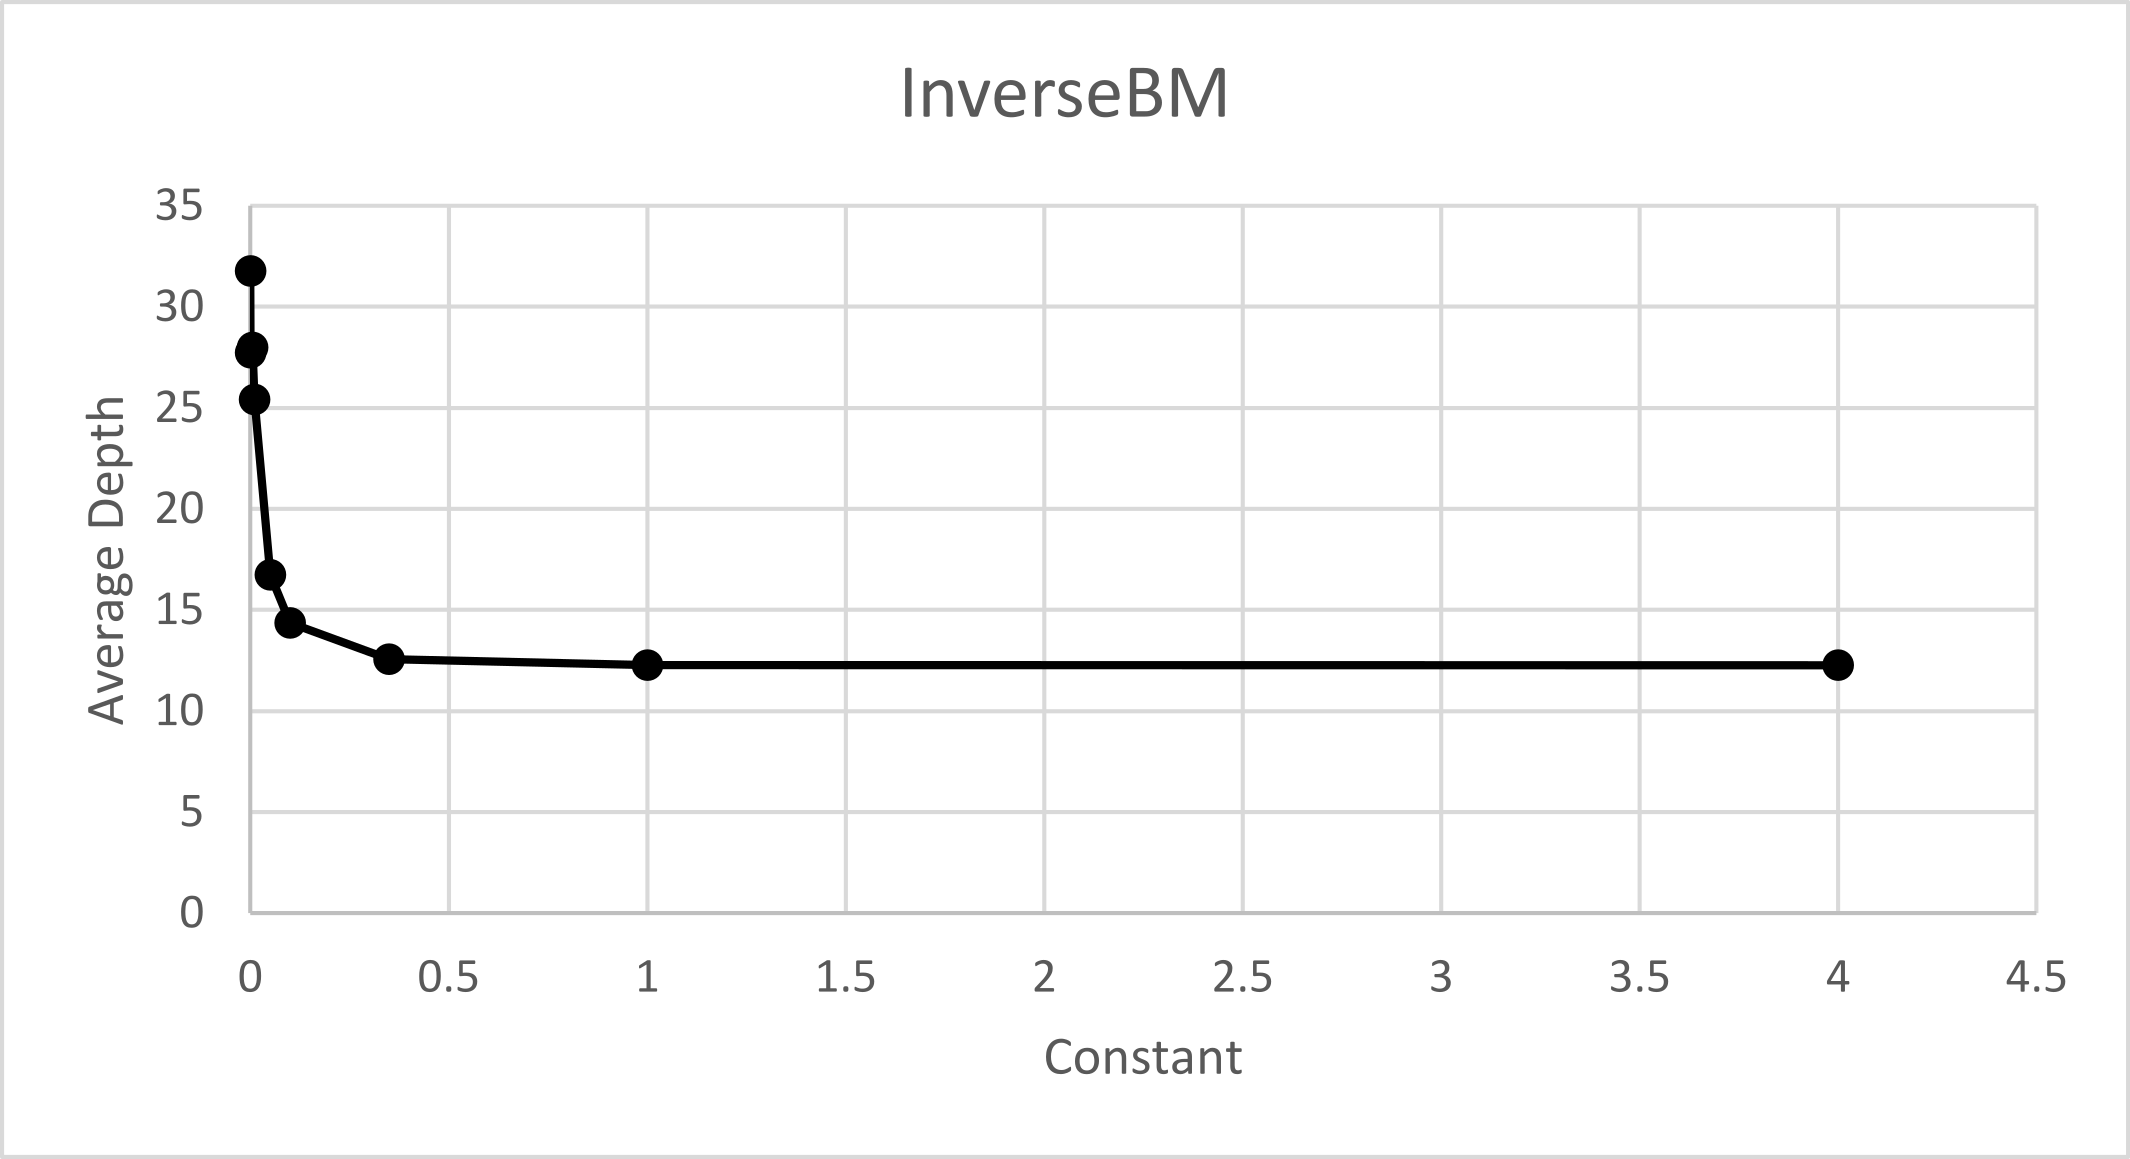
\includegraphics[width=0.8\linewidth]{pictures/InverseDepth.png}}
\subfigure[Trend of solved levels rate using different constant values for reward InverseBM]{
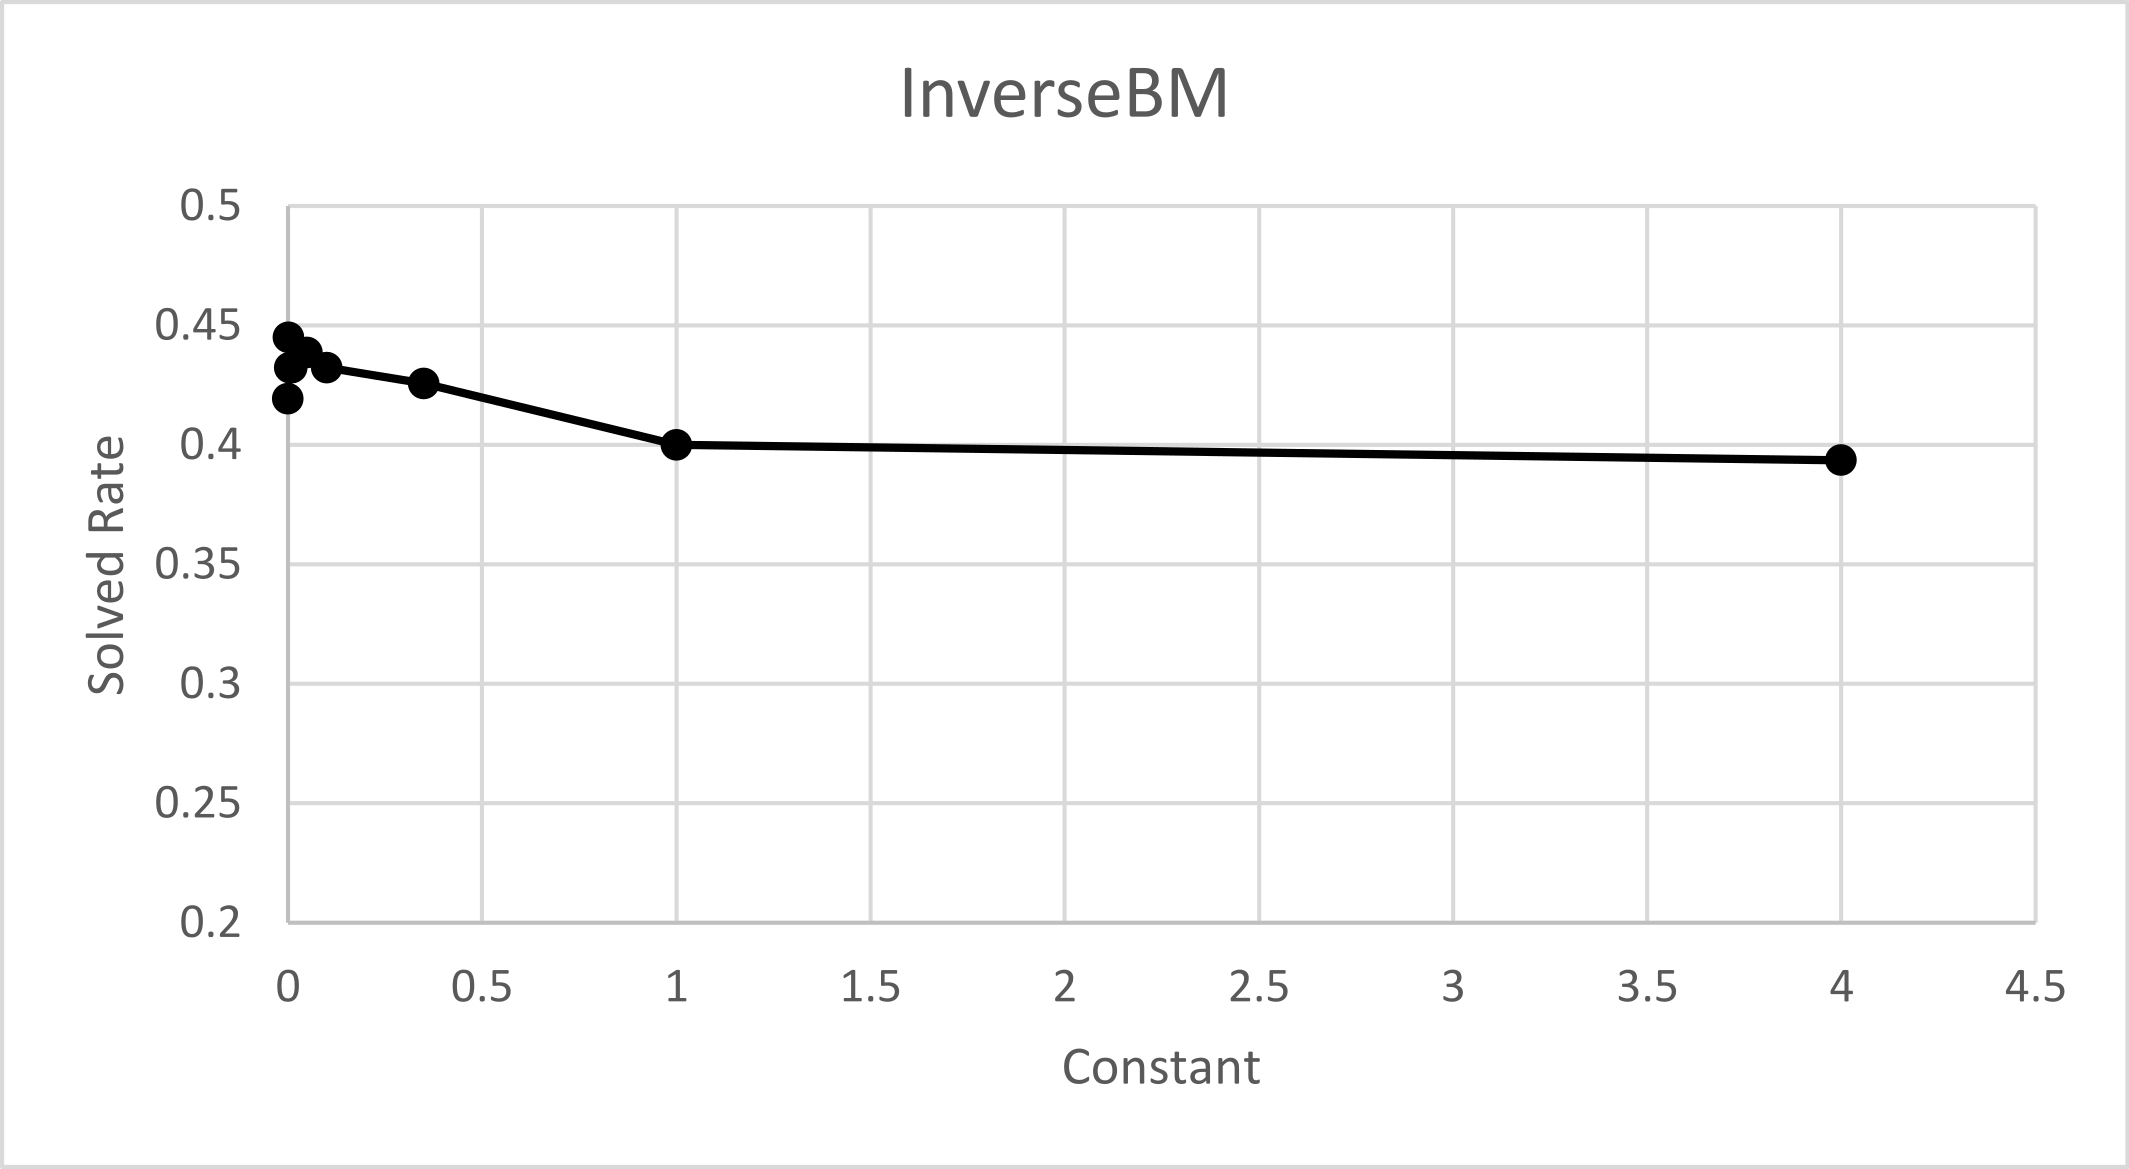
\includegraphics[width=0.8\linewidth]{pictures/InverseSolved.png}}
\caption[InverseBM solved levels rate and tree depth]{}
\label{fig:constant_InverseBM}
\end{figure}
\clearpage

\begin{figure}[!h]
\centering
\subfigure[Trend of generated tree depth using different constant values for reward NegativeBM]{
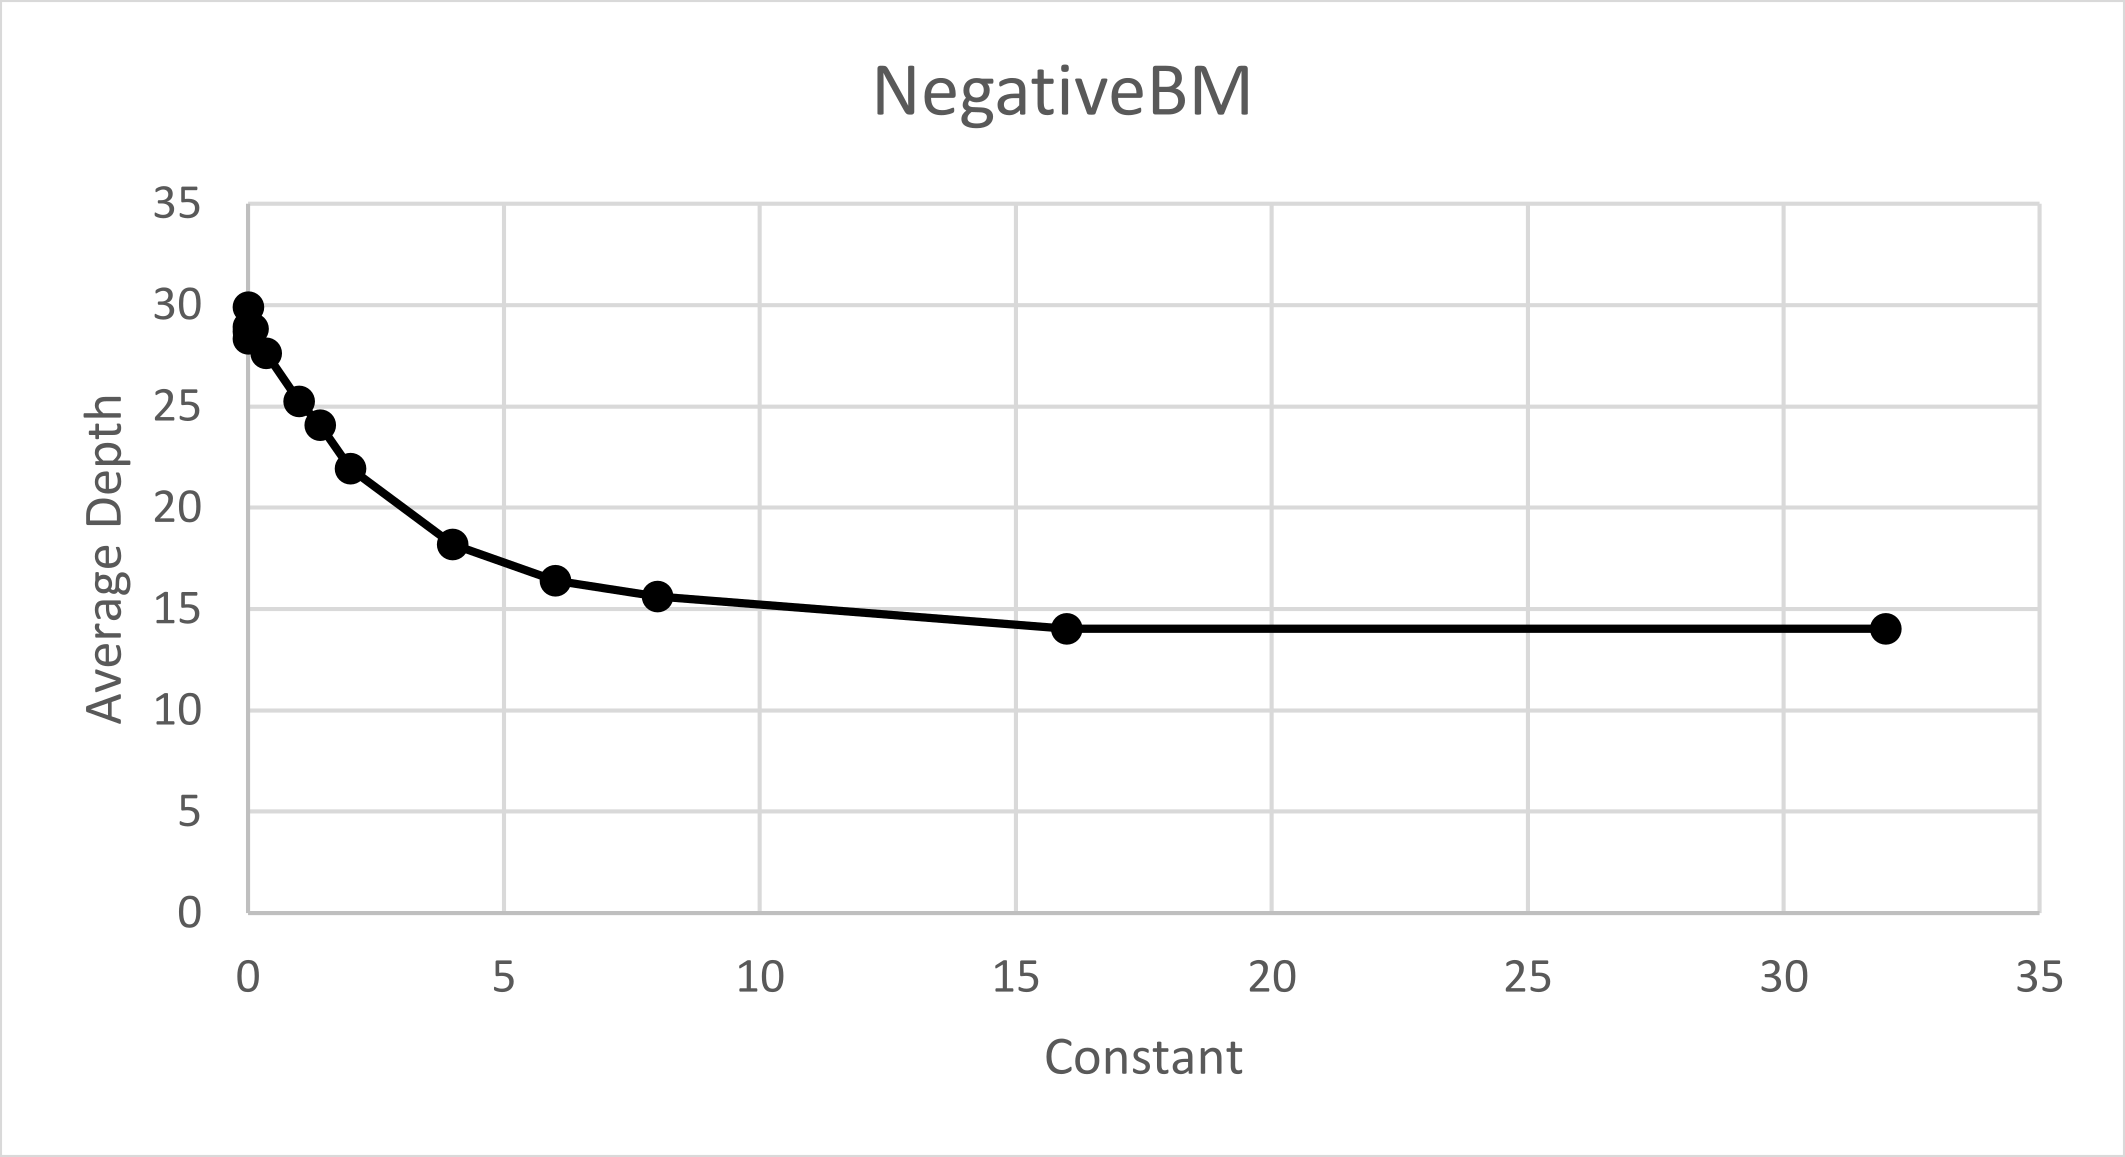
\includegraphics[width=0.8\linewidth]{pictures/NegativeDepth.png}}
\subfigure[Trend of solved levels rate using different constant values for reward NegativeBM]{
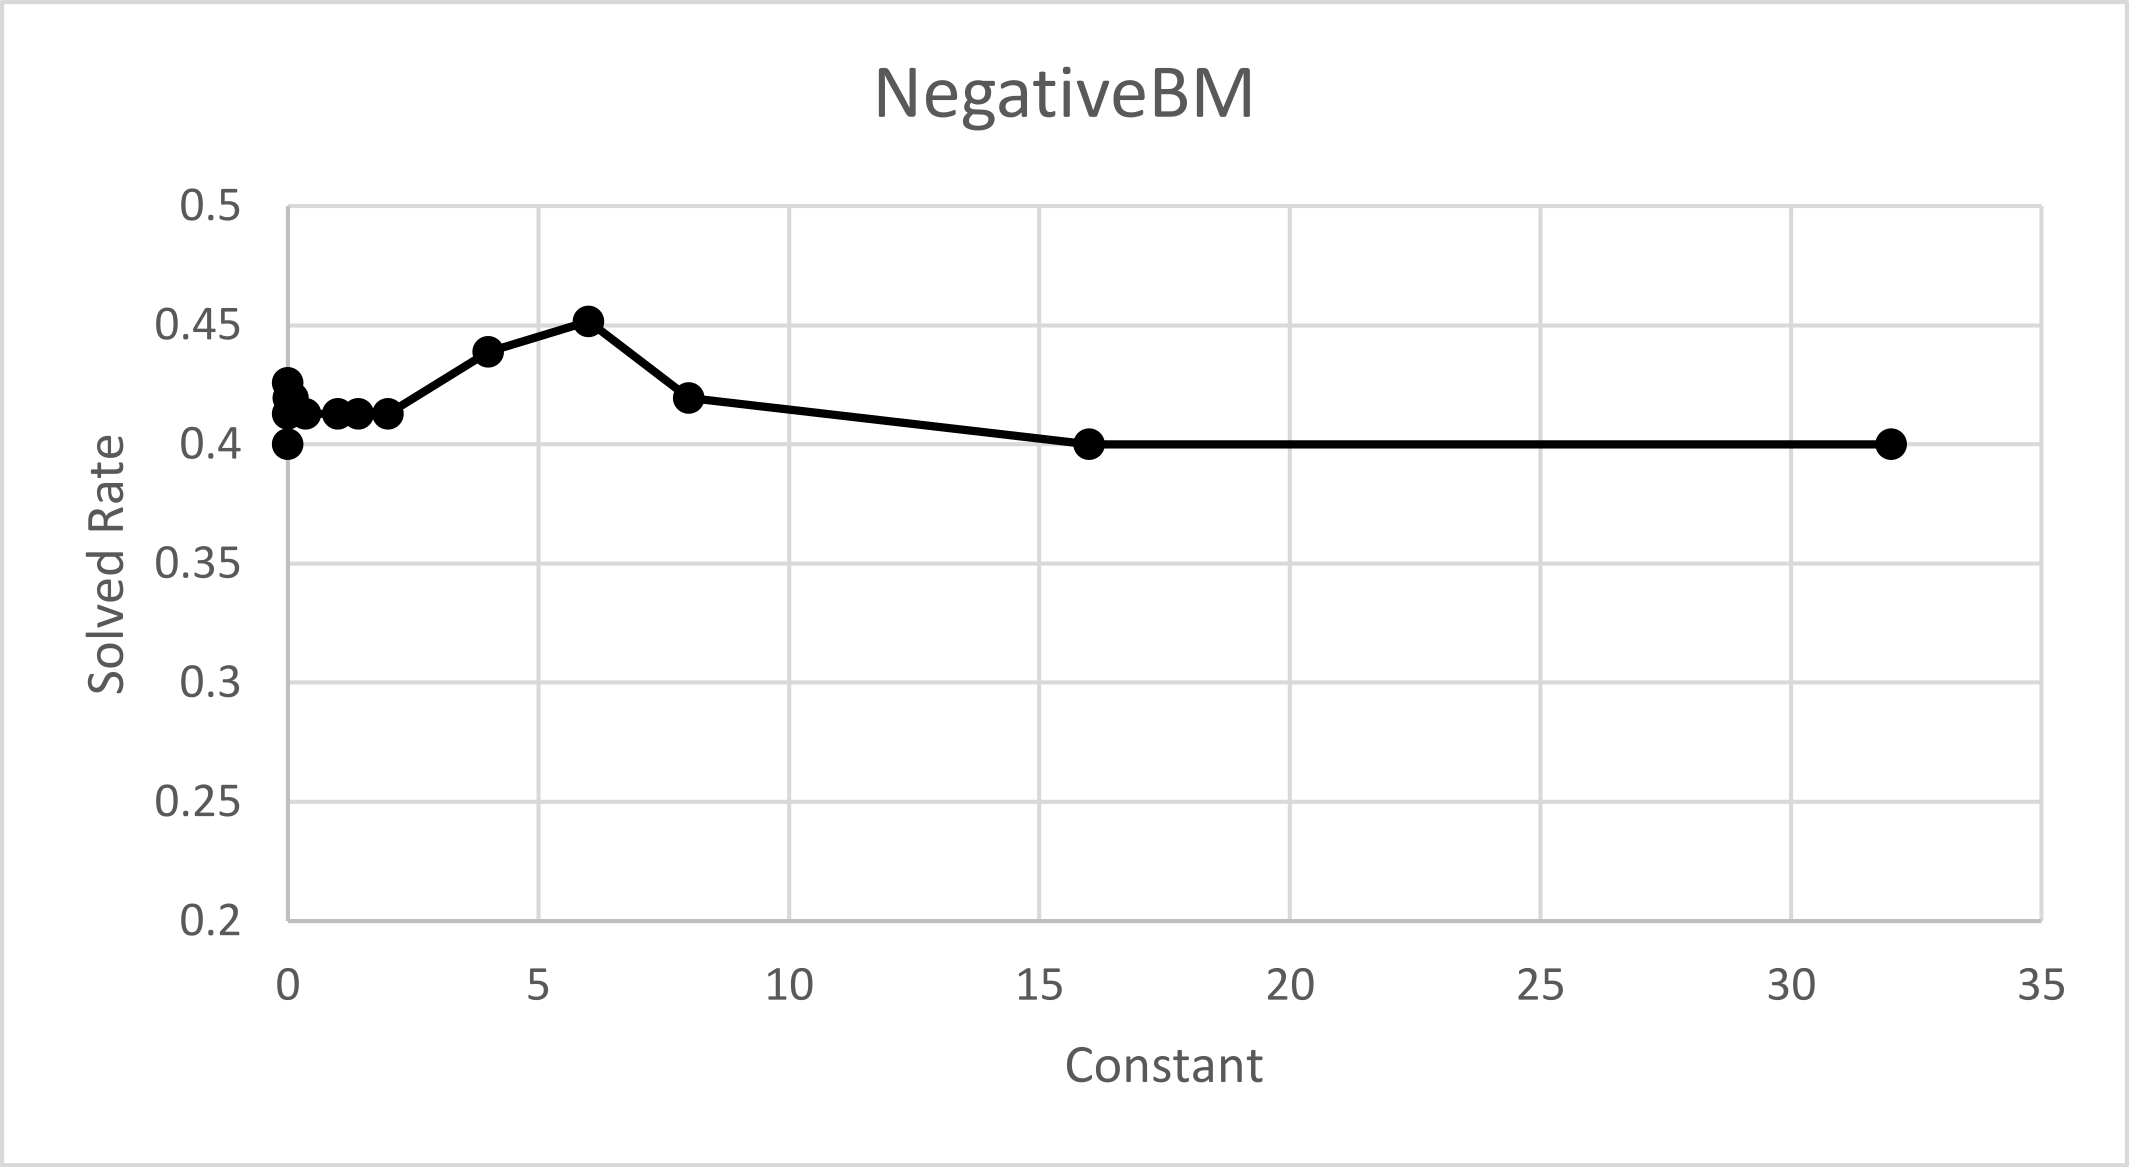
\includegraphics[width=0.8\linewidth]{pictures/NegativeSolved.png}}
\caption[NegativeBM solved levels rate and tree depth]{}
\label{fig:constant_NegativeBM}
\end{figure}

\medskip\noindent
NegativeBM reaches its maximum score with a constant value of 6 and the generated tree depth decreases more gradually due to the larger reward range.
\clearpage

\begin{figure}[!h]
\centering
\subfigure[Trend of generated tree depth using different constant values for reward R0]{
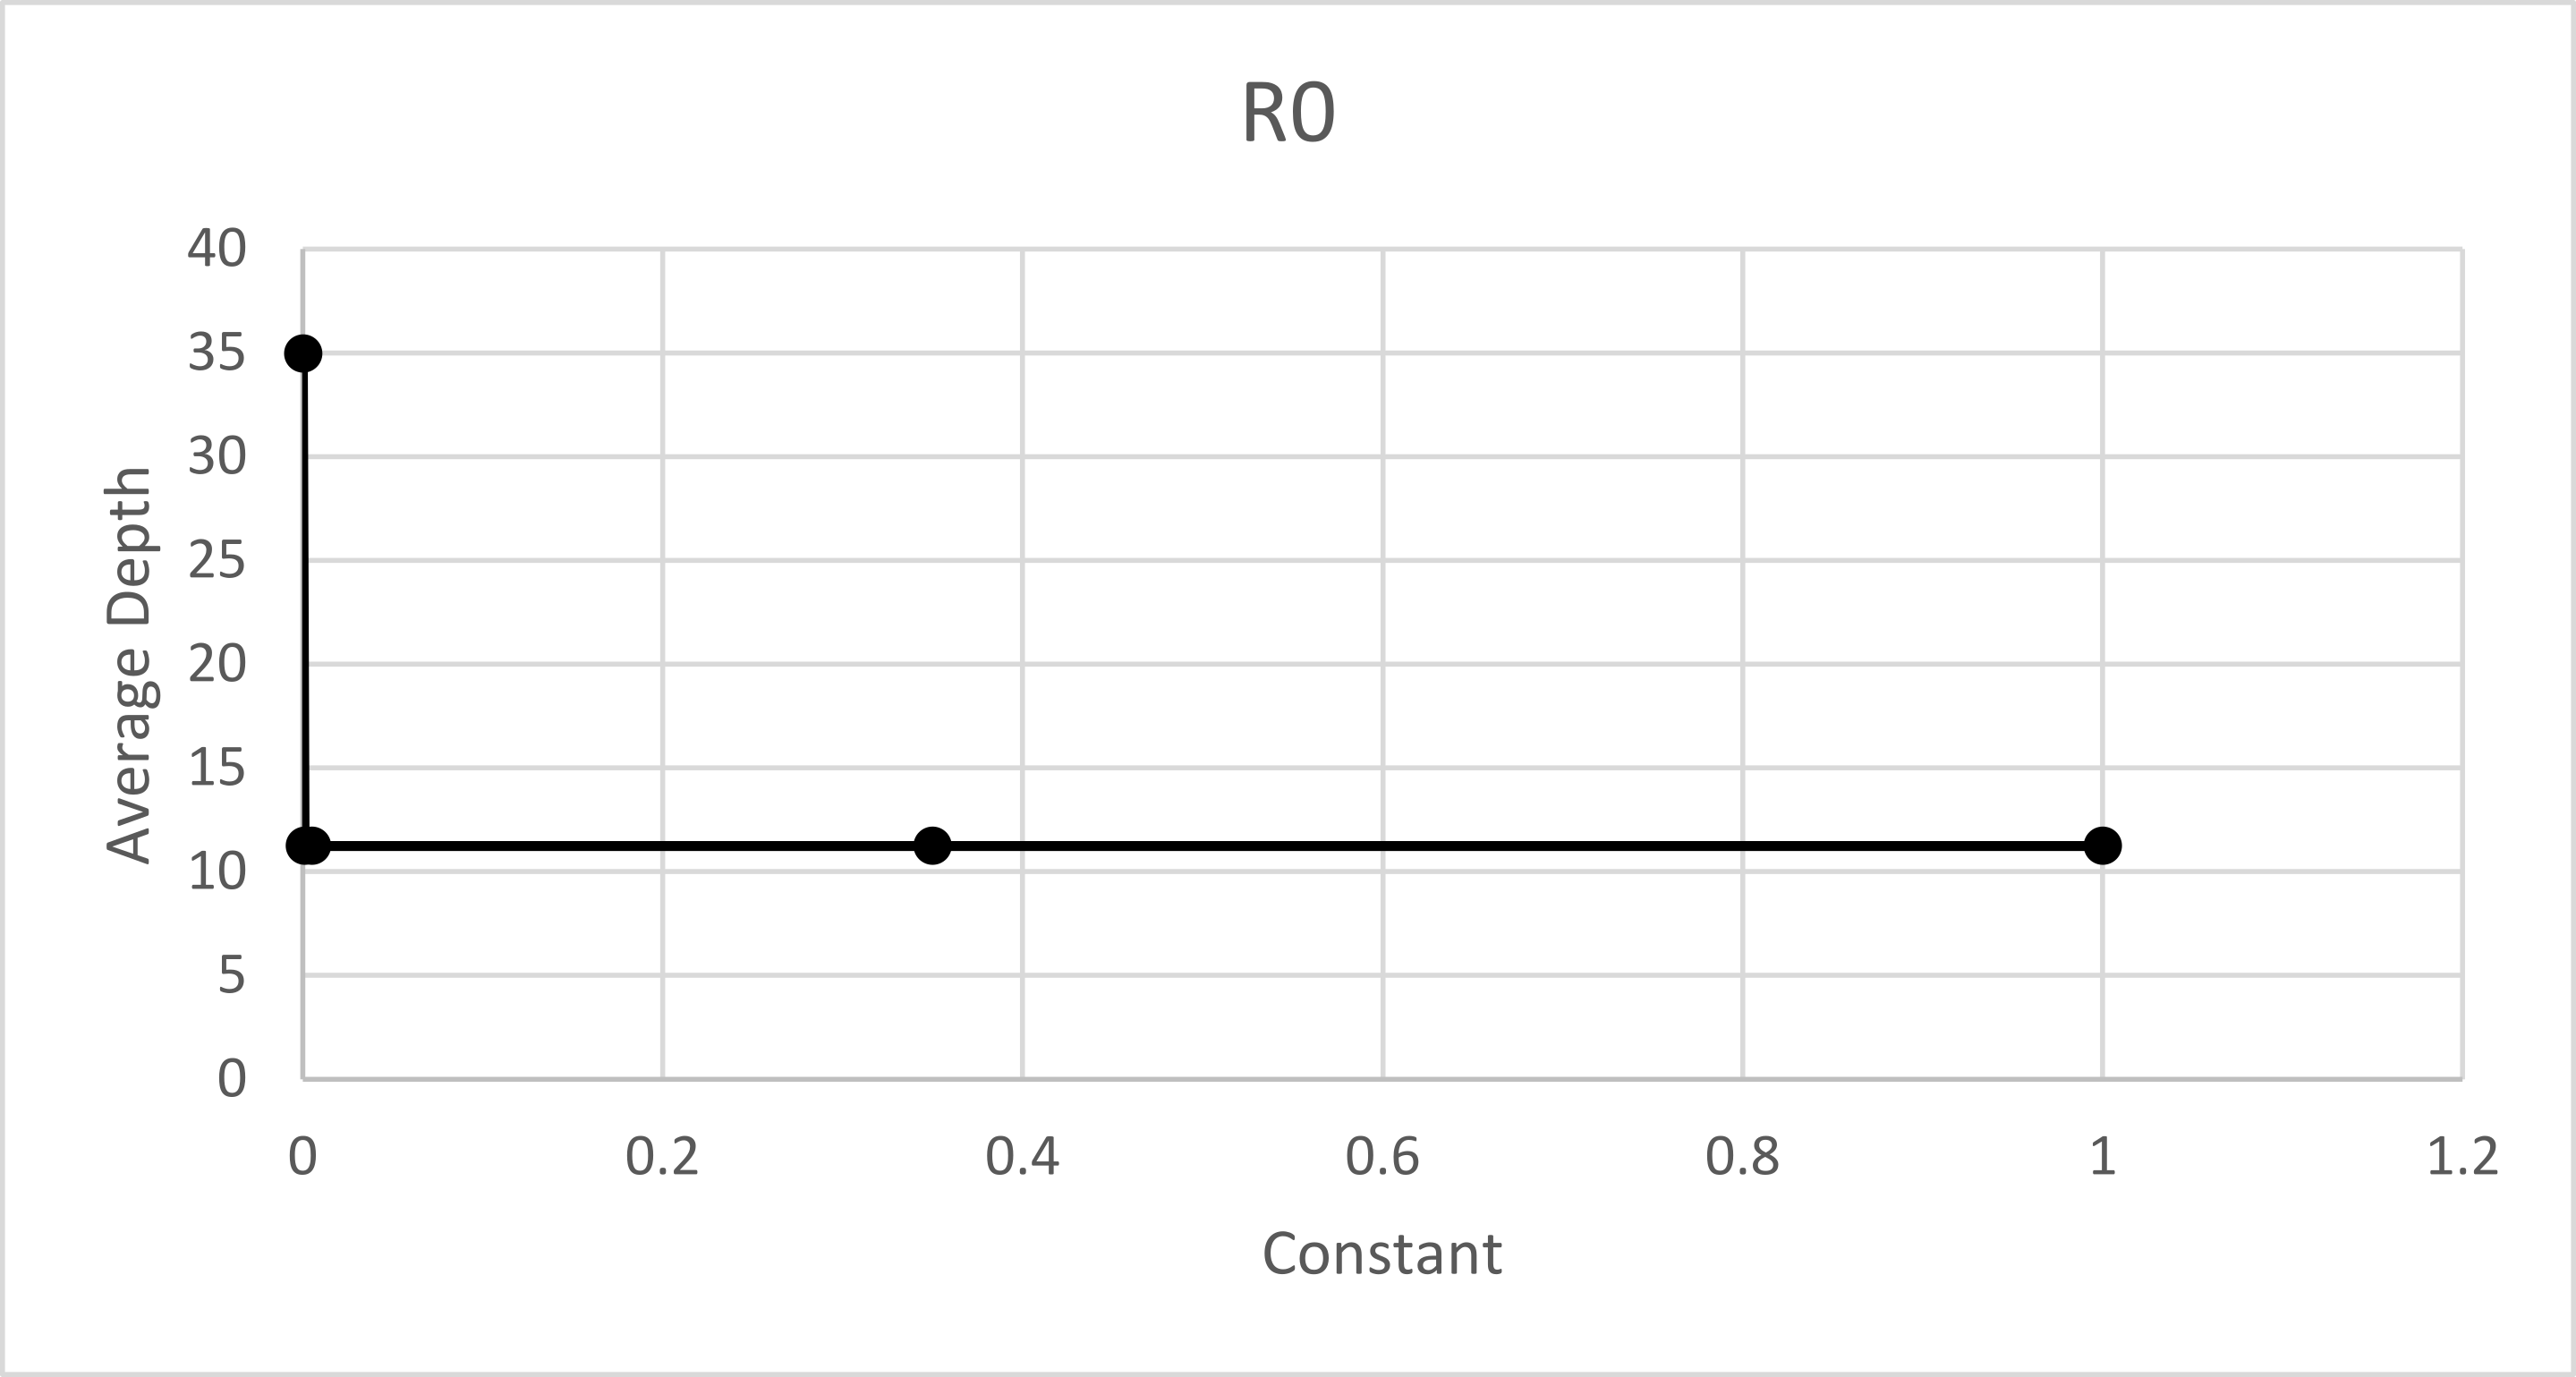
\includegraphics[width=0.8\linewidth]{pictures/R0Depth.png}}
\subfigure[Trend of solved levels rate using different constant values for reward R0]{
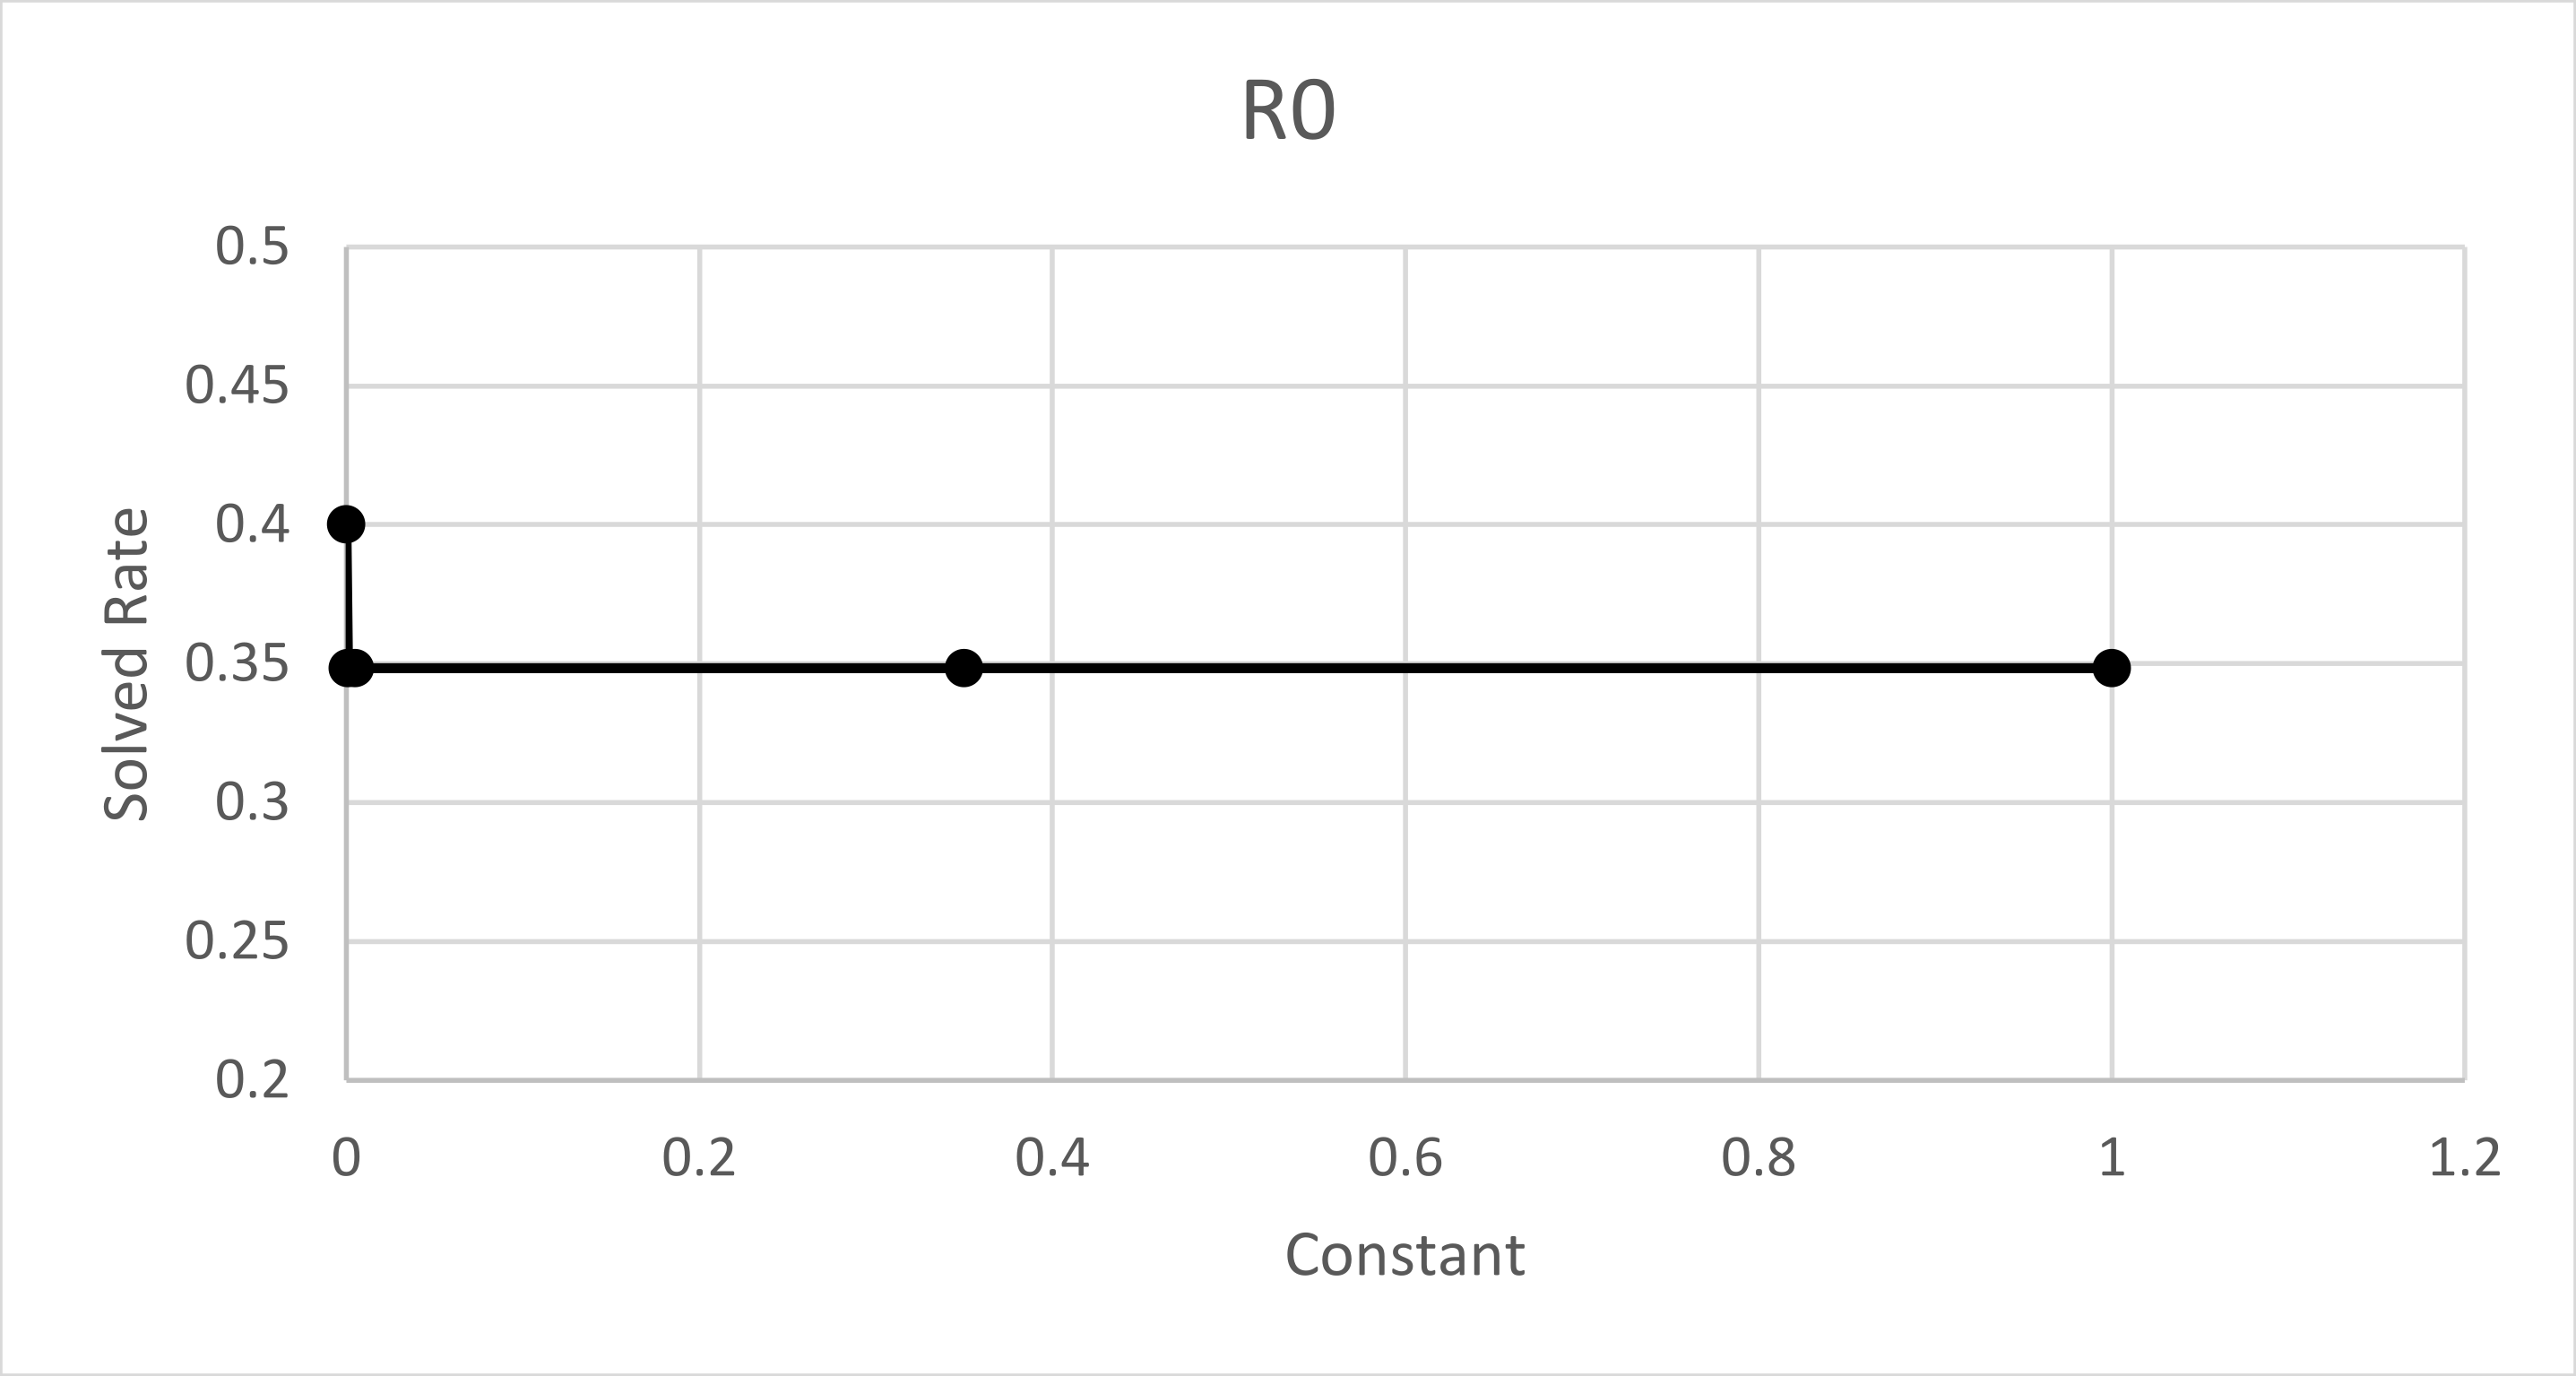
\includegraphics[width=0.8\linewidth]{pictures/R0Solved.png}}
\caption[R0 solved levels rate and tree depth]{}
\label{fig:constant_R0}
\end{figure}

\medskip\noindent
R0 charts clearly show how this reward type is not suitable for solving Sokoban using MCTS. The depth of the trees confirms what we suspected: with the reward being 0 for every rollout except for the last one (since the search is stopped at the first solution), the only relevant part of the UCT formula is the exploration component, which means that for every value of the constant greater than 0, the algorithm will perform a pure exploration. In our implementation if two or more nodes have the same UCT value, the selection phase is deterministic and always chooses the node that was generated first. This implies that with the constant equal to 0, all nodes have a UCT value of 0 and the algorithm will perform a pure exploitation.

\begin{figure}[!h]
\centering
\subfigure[Trend of generated tree depth using different constant values for reward Boxes]{
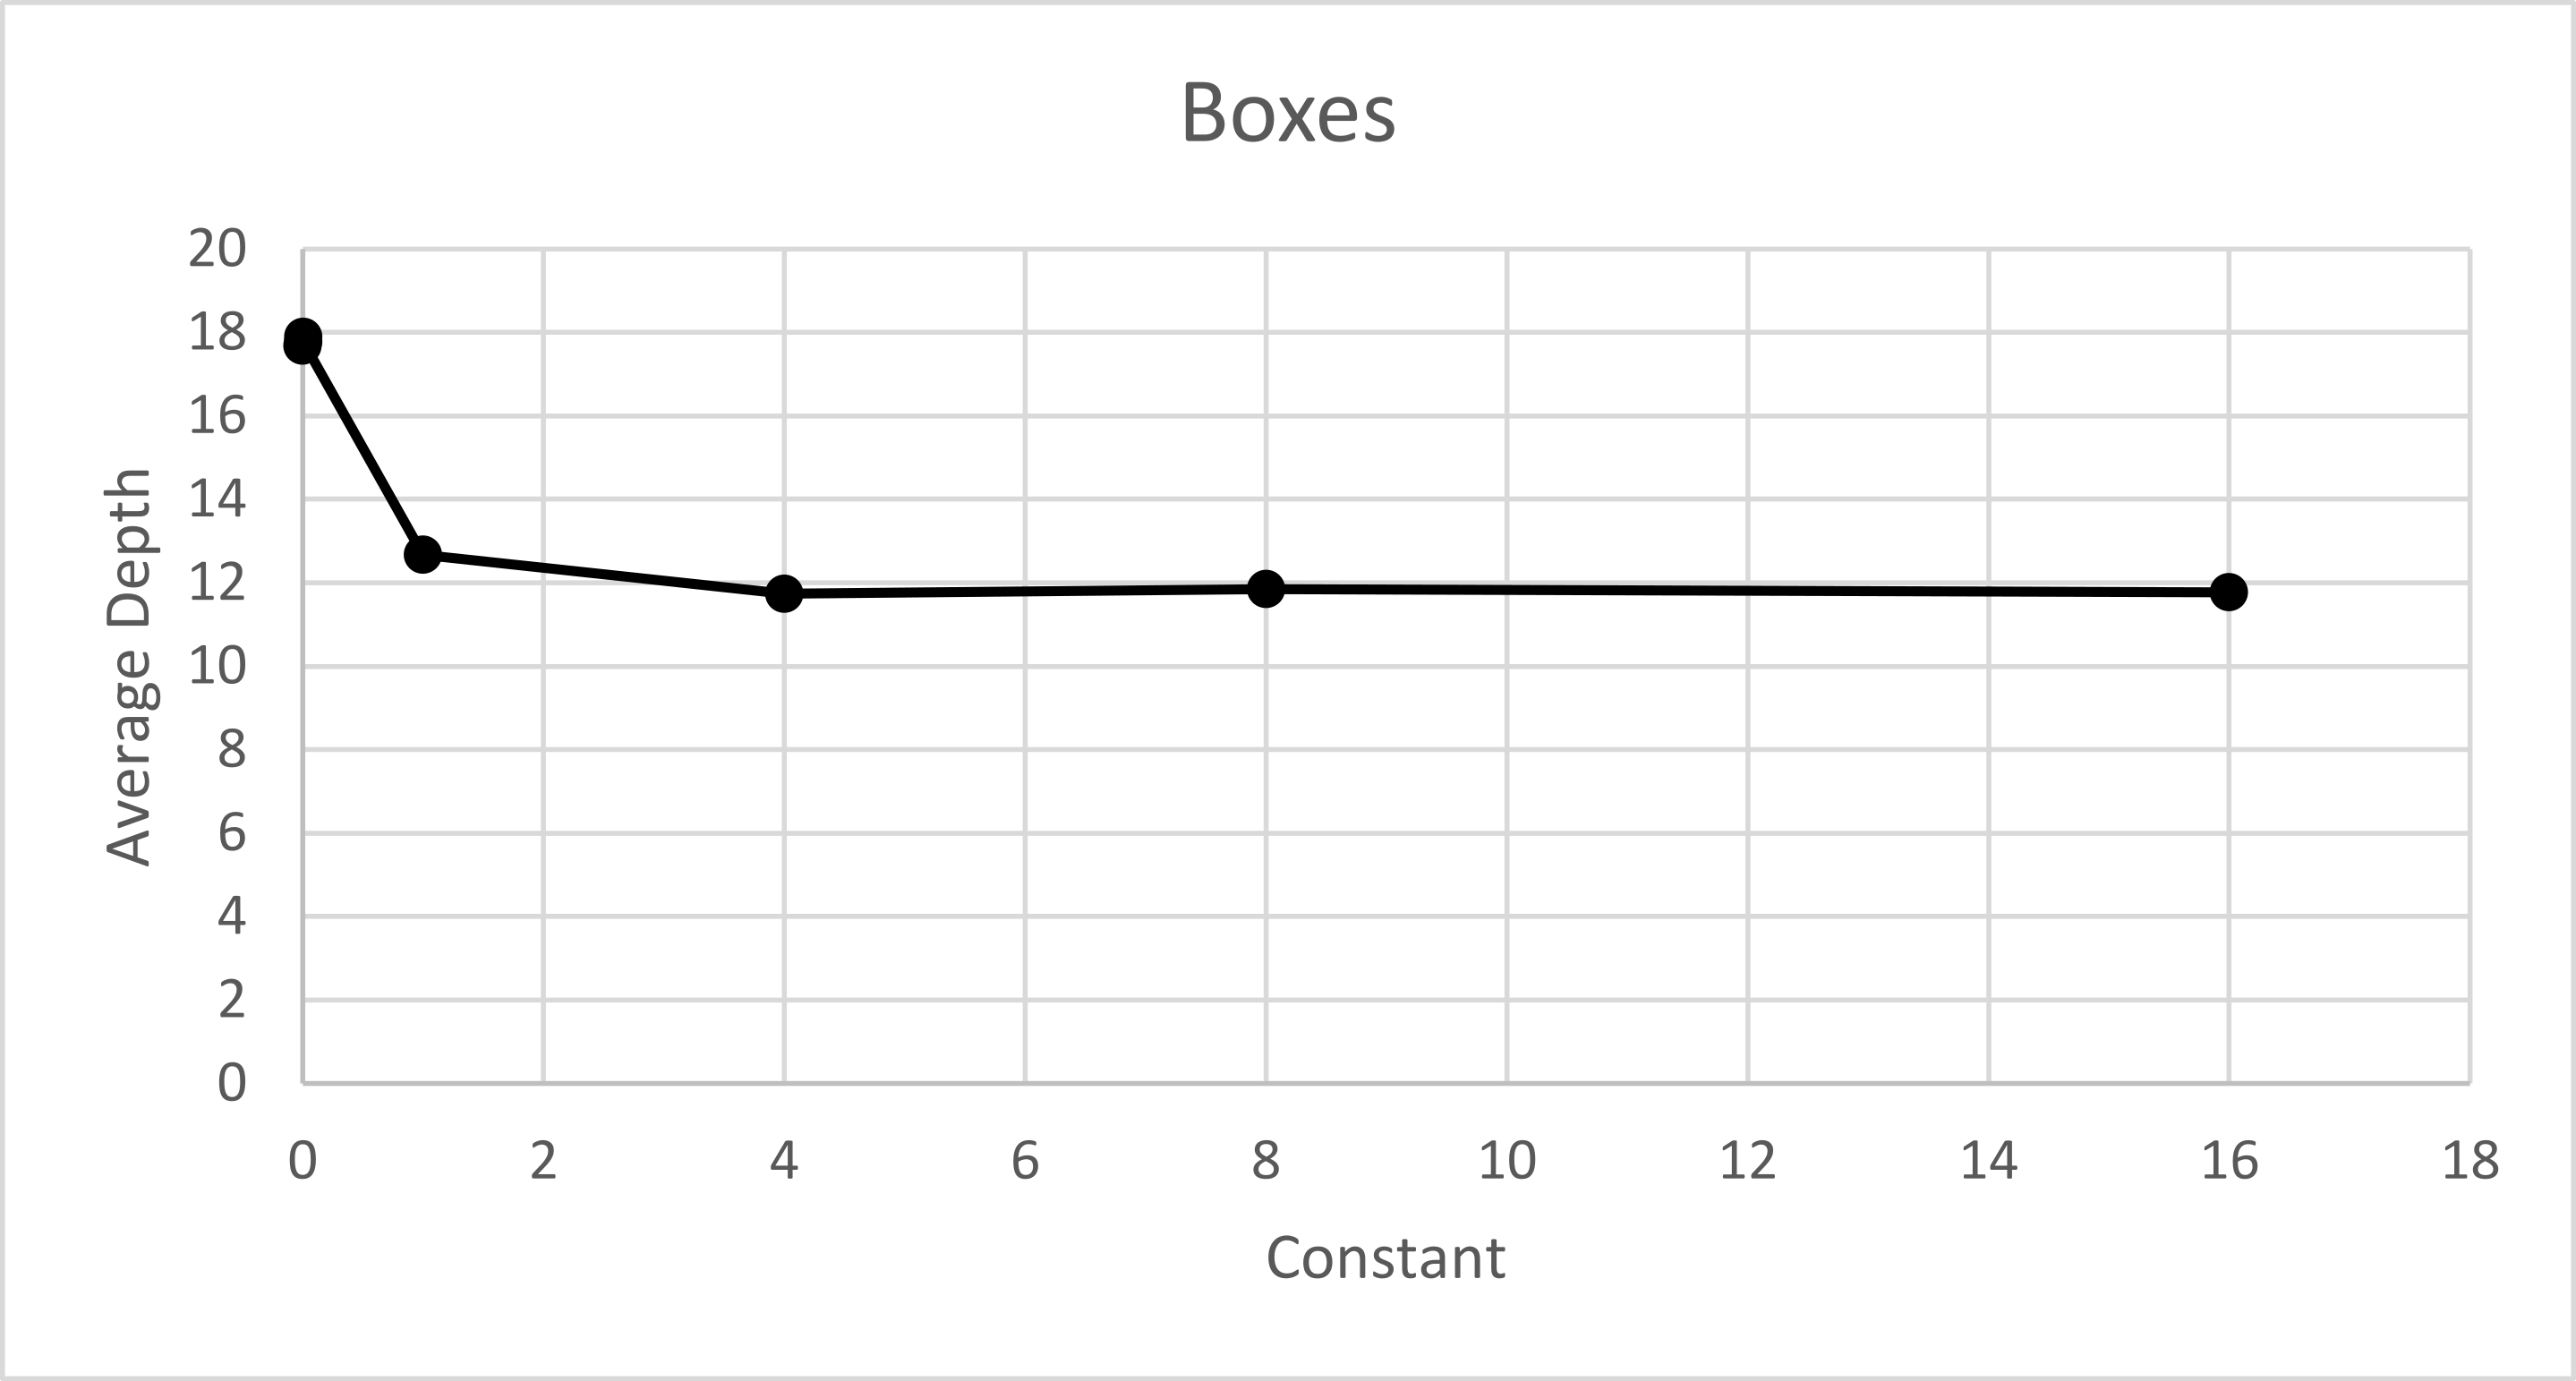
\includegraphics[width=0.8\linewidth]{pictures/BoxesDepth.png}}
\subfigure[Trend of solved levels rate using different constant values for reward Boxes]{
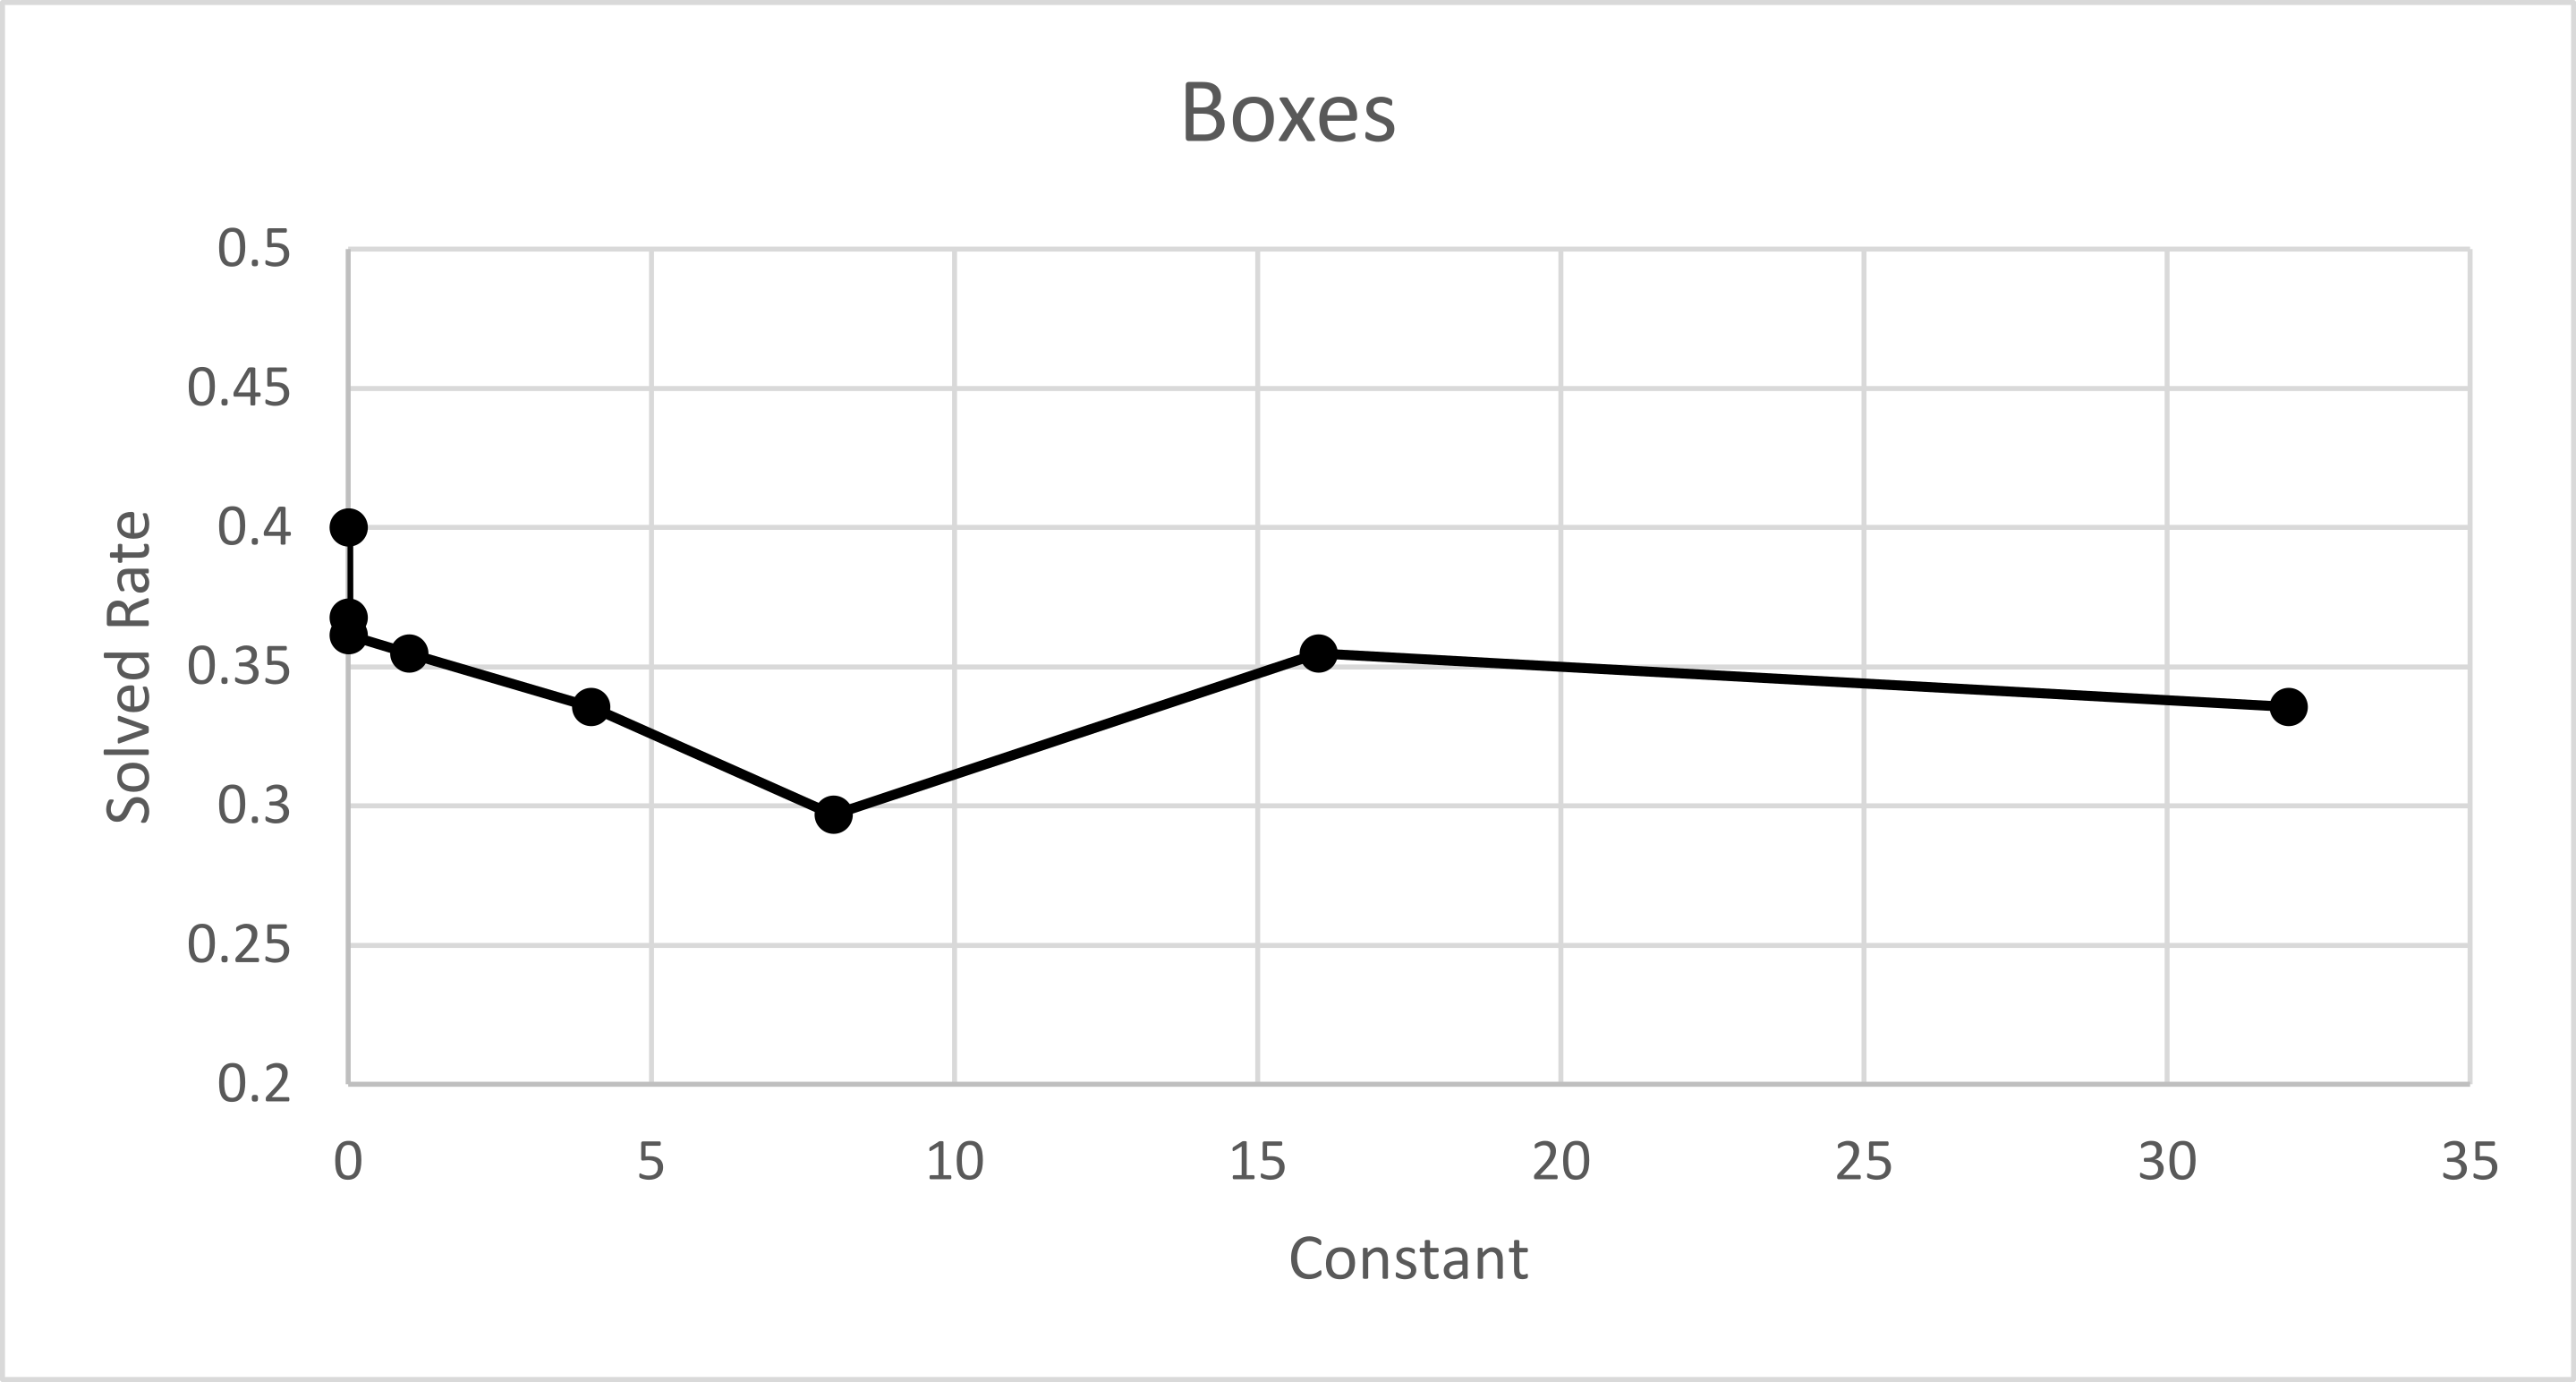
\includegraphics[width=0.8\linewidth]{pictures/BoxesSolved.png}}
\caption[Boxes solved levels rate and tree depth]{}
\label{fig:constant_Boxes}
\end{figure}

\medskip\noindent
The results using Boxes reward do not seem to follow a specific trend, and with the top score obtained with the constant equal to 0, this too does not appear to be suitable for solving Sokoban with MCTS.

\medskip\noindent
Considering these results, we selected NegativeBM as a reward for the following experiments.

\medskip\noindent
We also performed the same experiments using SP-MCTS and UCB1-Tuned to determine the best reward and constant configuration for each. The results are shown in Figures \ref{fig:spmcts_inverse} through \ref{fig:spmcts_R0}. SP-MCTS reached its peak performance with NegativeBM and a constant of 2, while UCB1-Tuned obtained the best result with InverseBM and a constant of 0.05.

\begin{figure}[!h]
    \centering
    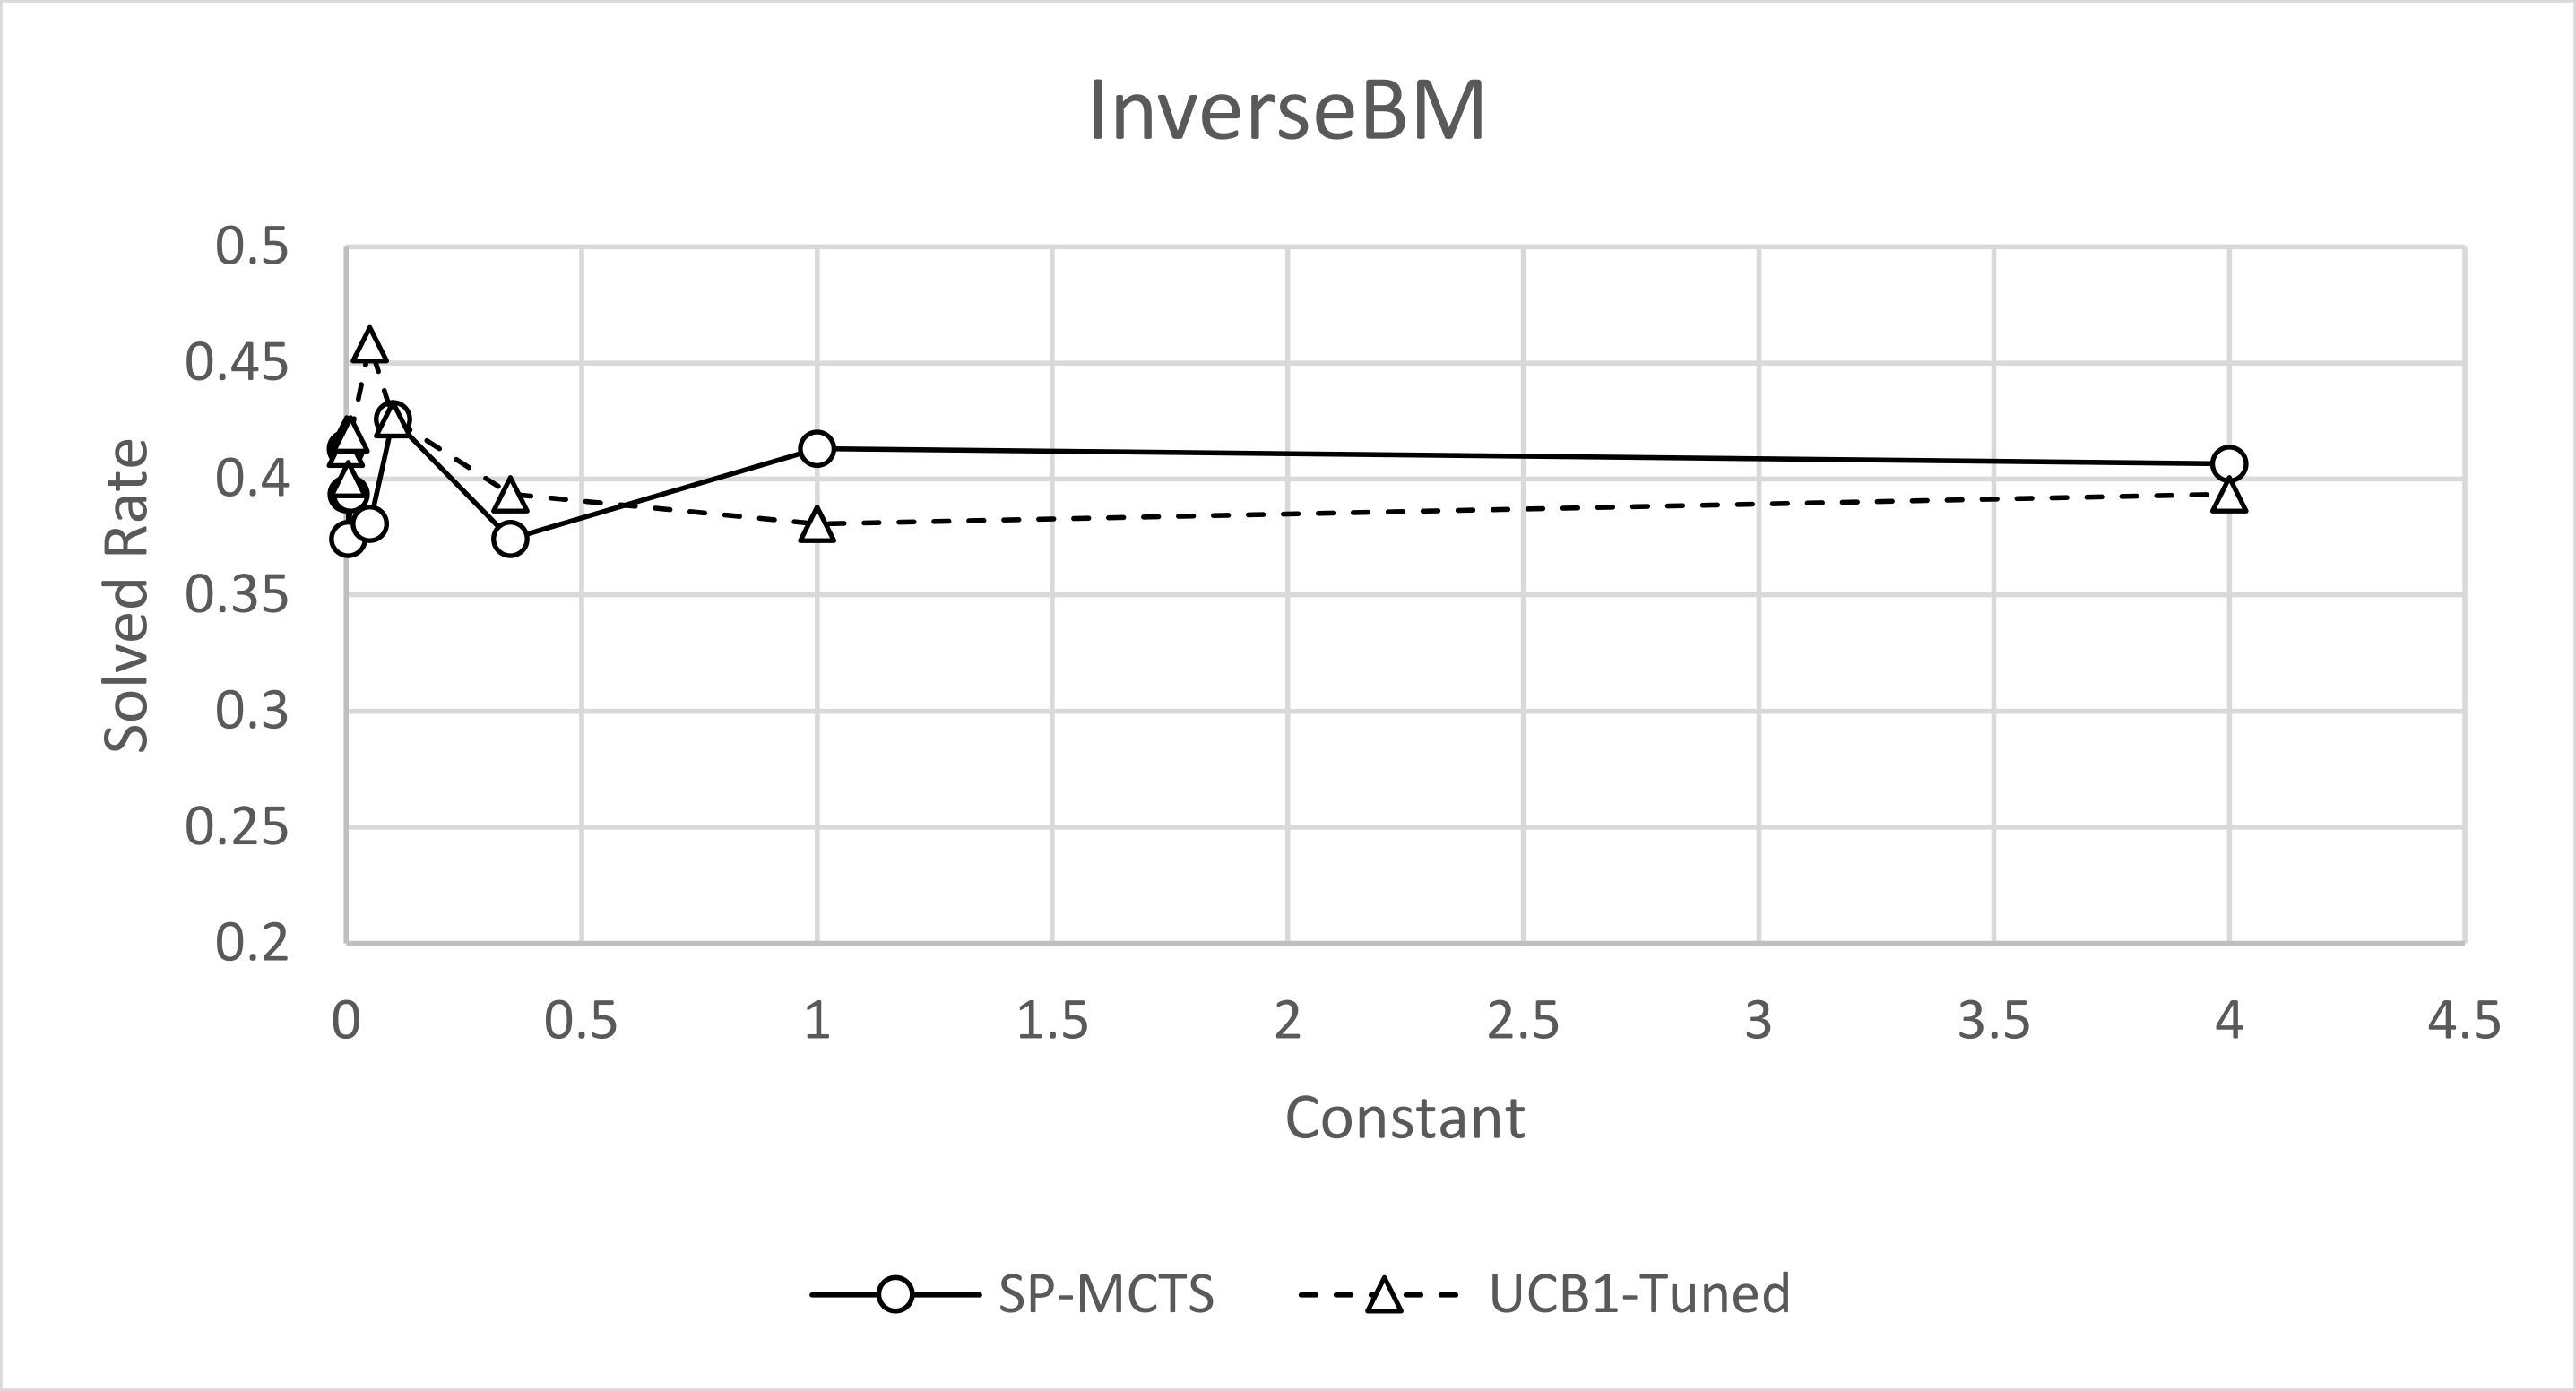
\includegraphics[width=0.8\linewidth]{pictures/Sokoban-SP-Inverse.png}
    \caption{SP-MCTS and UCB1-Tuned results with InverseBM}
    \label{fig:spmcts_inverse}
\end{figure}

\begin{figure}[!h]
    \centering
    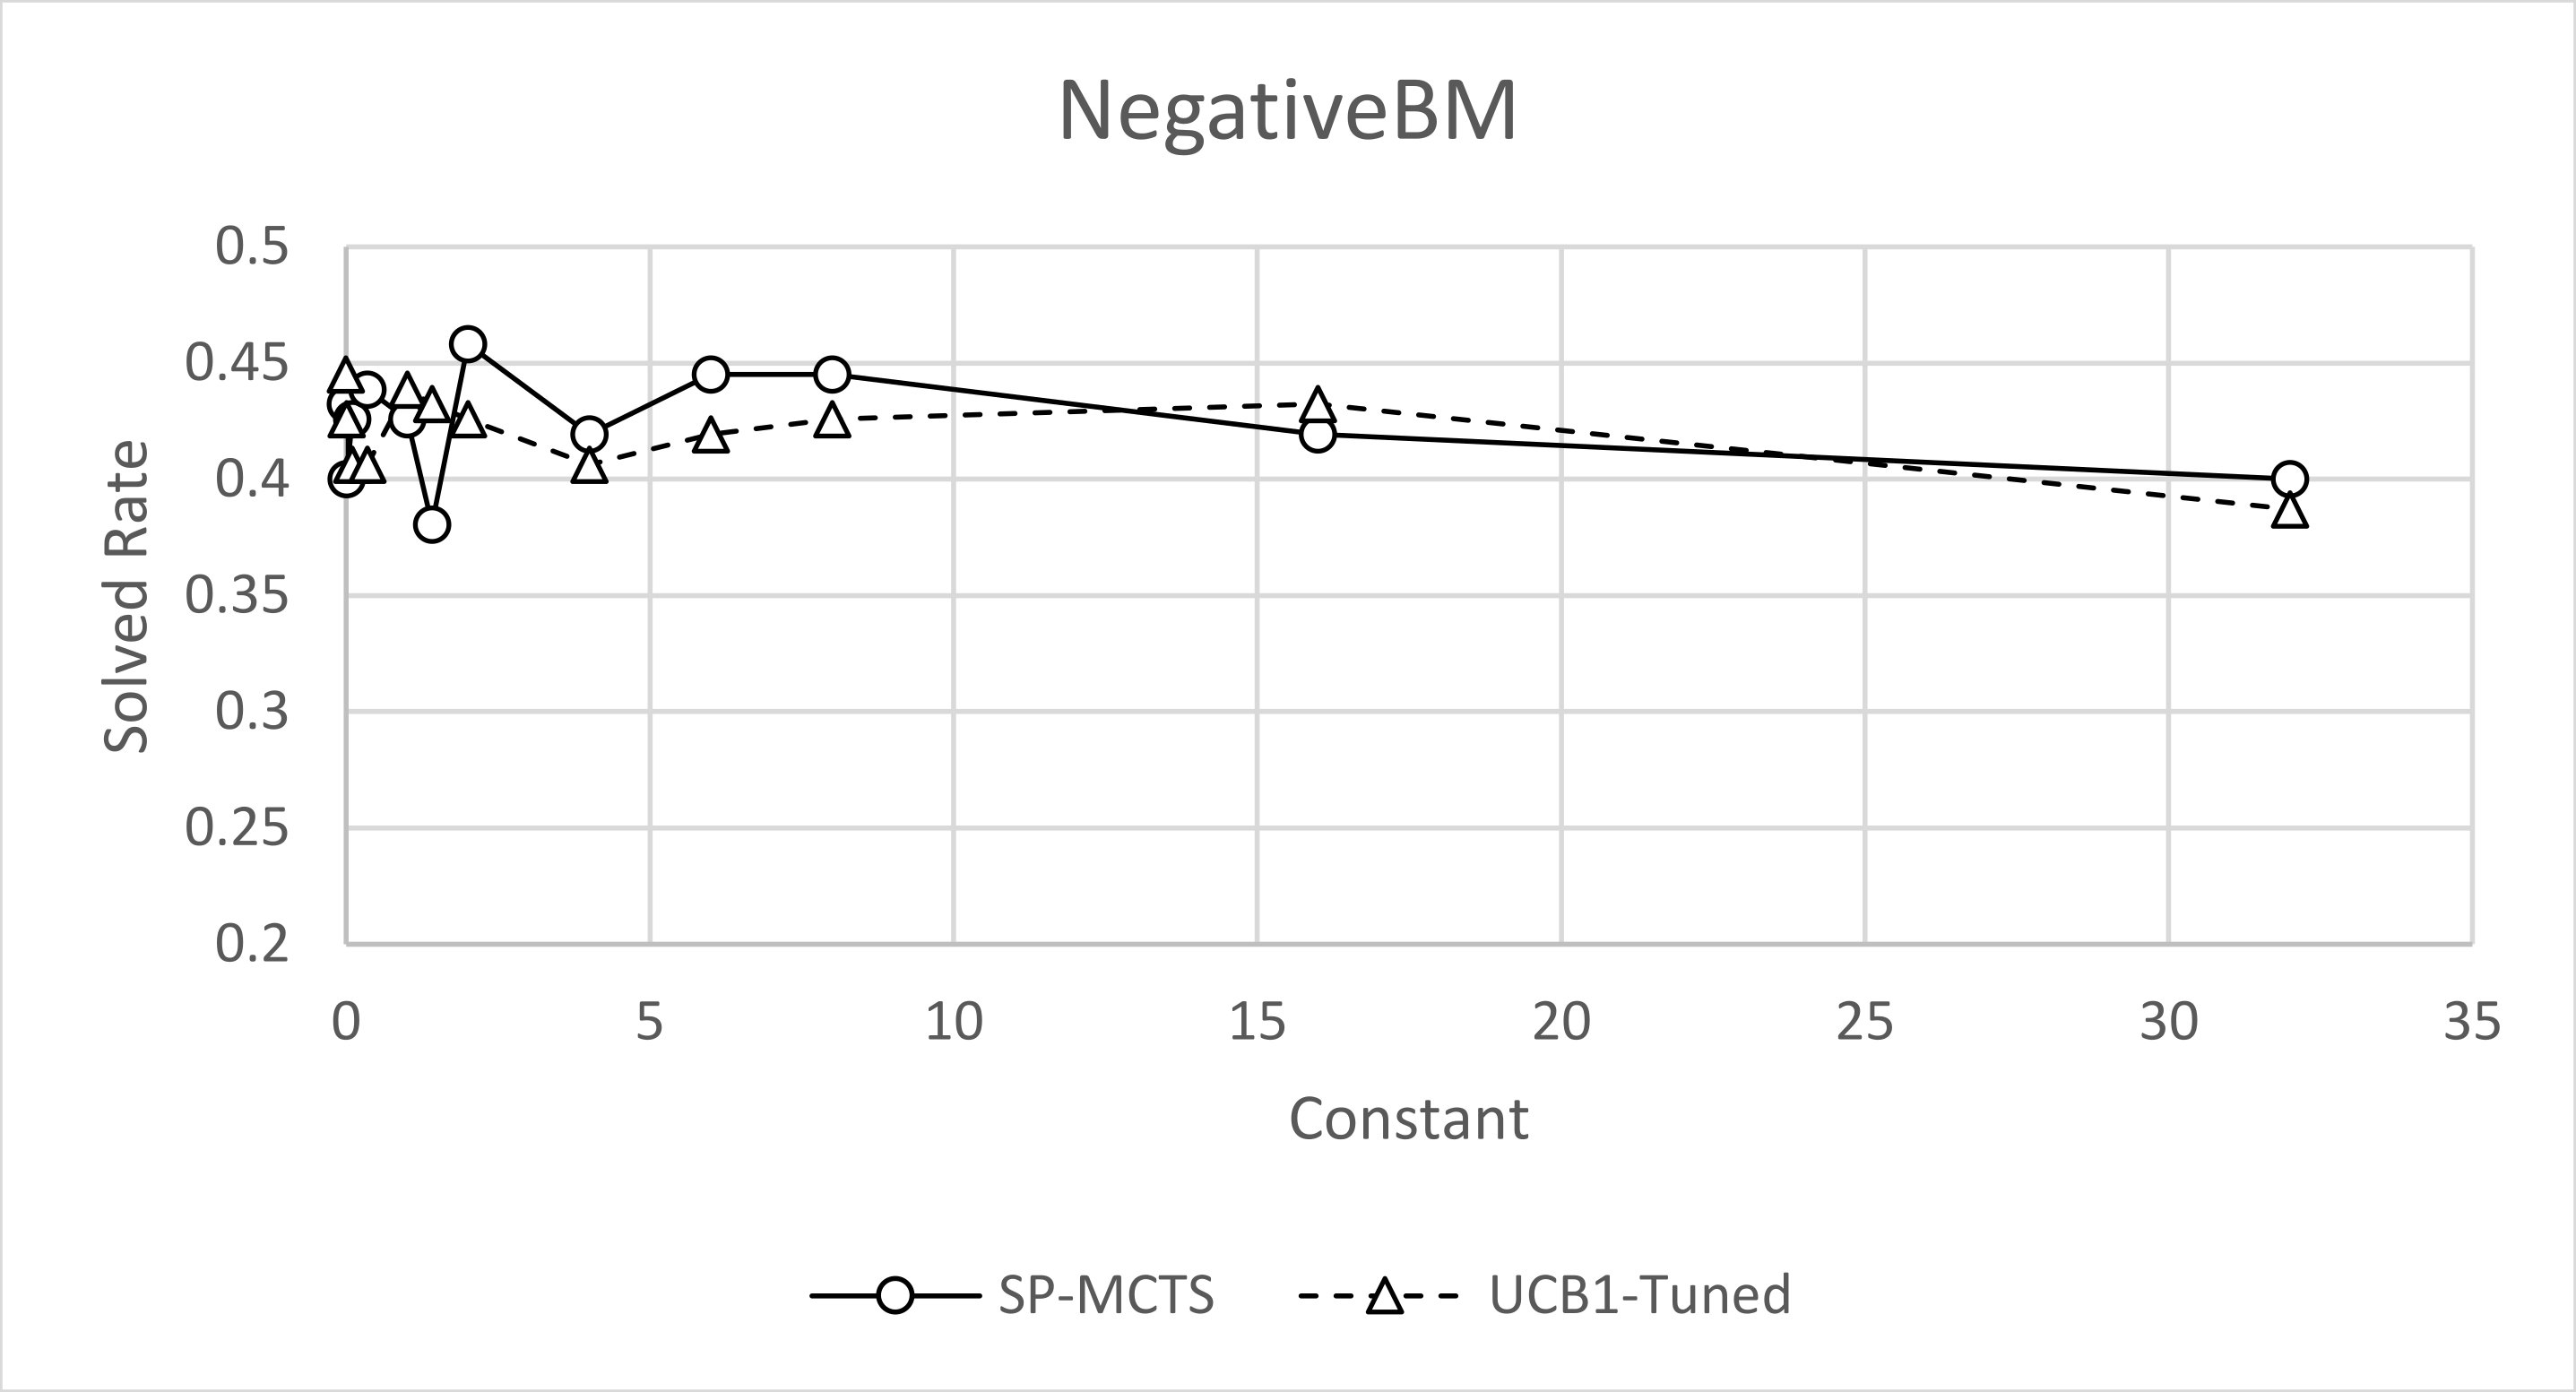
\includegraphics[width=0.8\linewidth]{pictures/Sokoban-SP-Negative.png}
    \caption{SP-MCTS and UCB1-Tuned results with NegativeBM}
    \label{fig:spmcts_negative}
\end{figure}

\clearpage

\begin{figure}[!h]
    \centering
    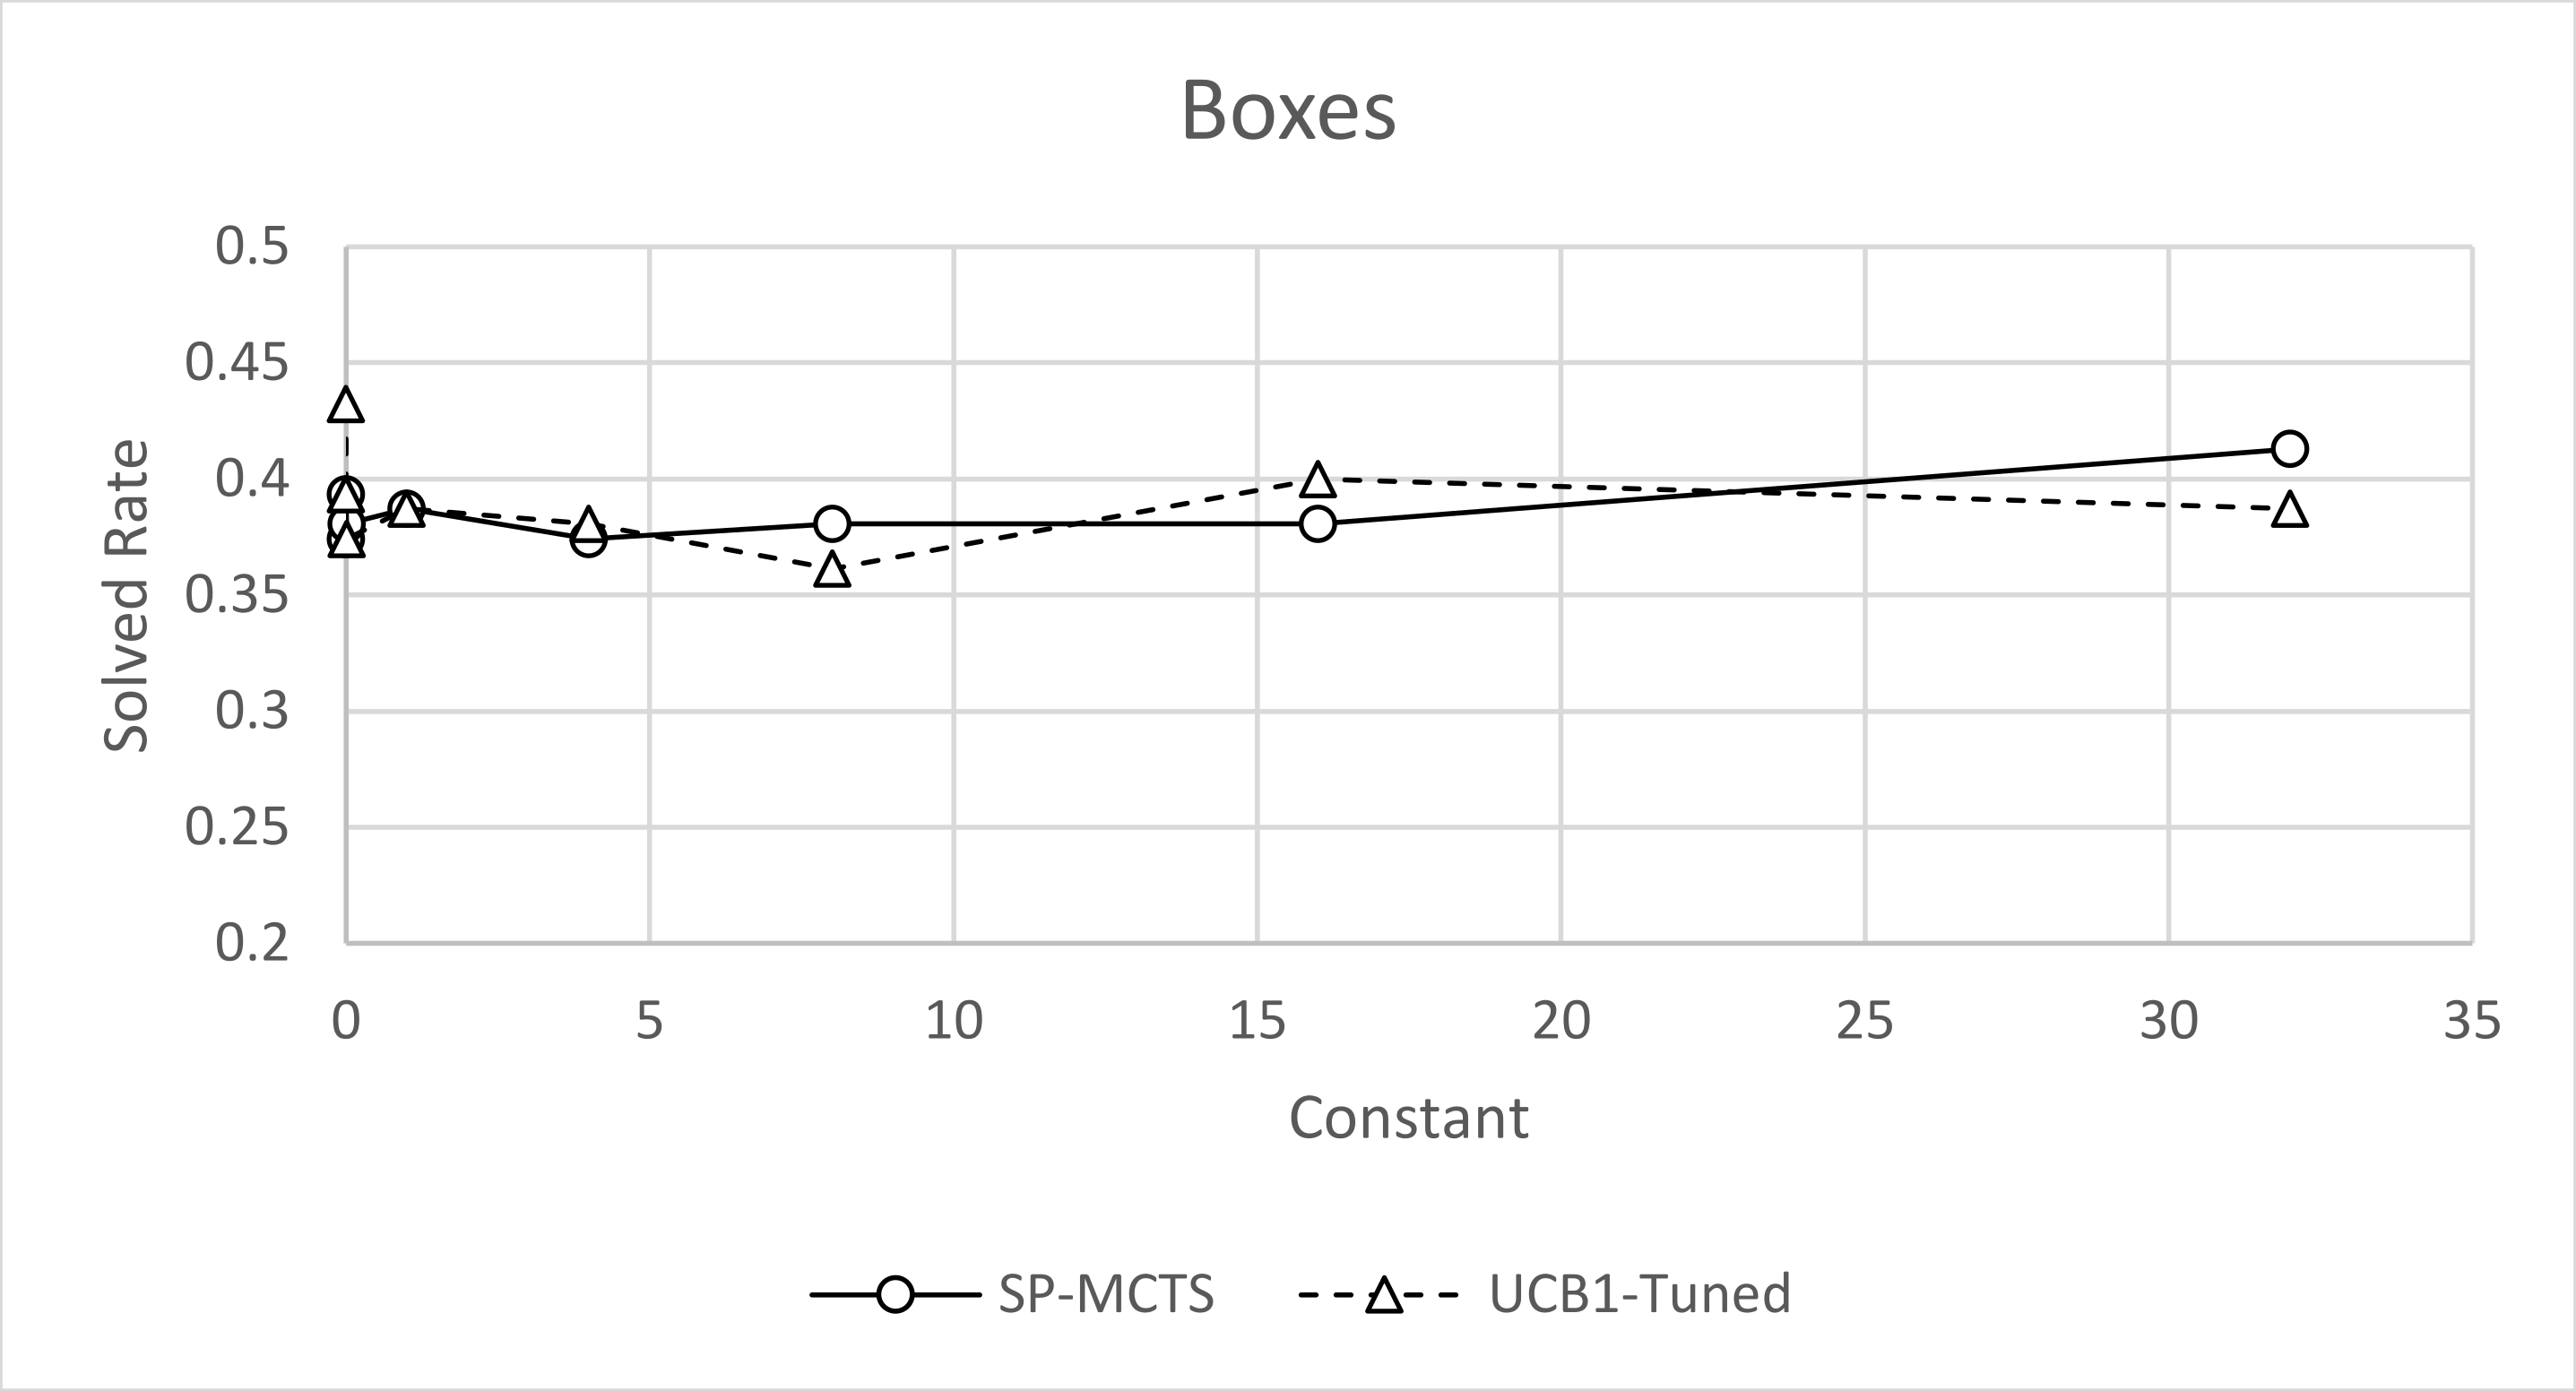
\includegraphics[width=0.8\linewidth]{pictures/Sokoban-SP-Boxes.png}
    \caption{SP-MCTS and UCB1-Tuned results with Boxes}
    \label{fig:spmcts_boxes}
\end{figure}

\begin{figure}[!h]
    \centering
    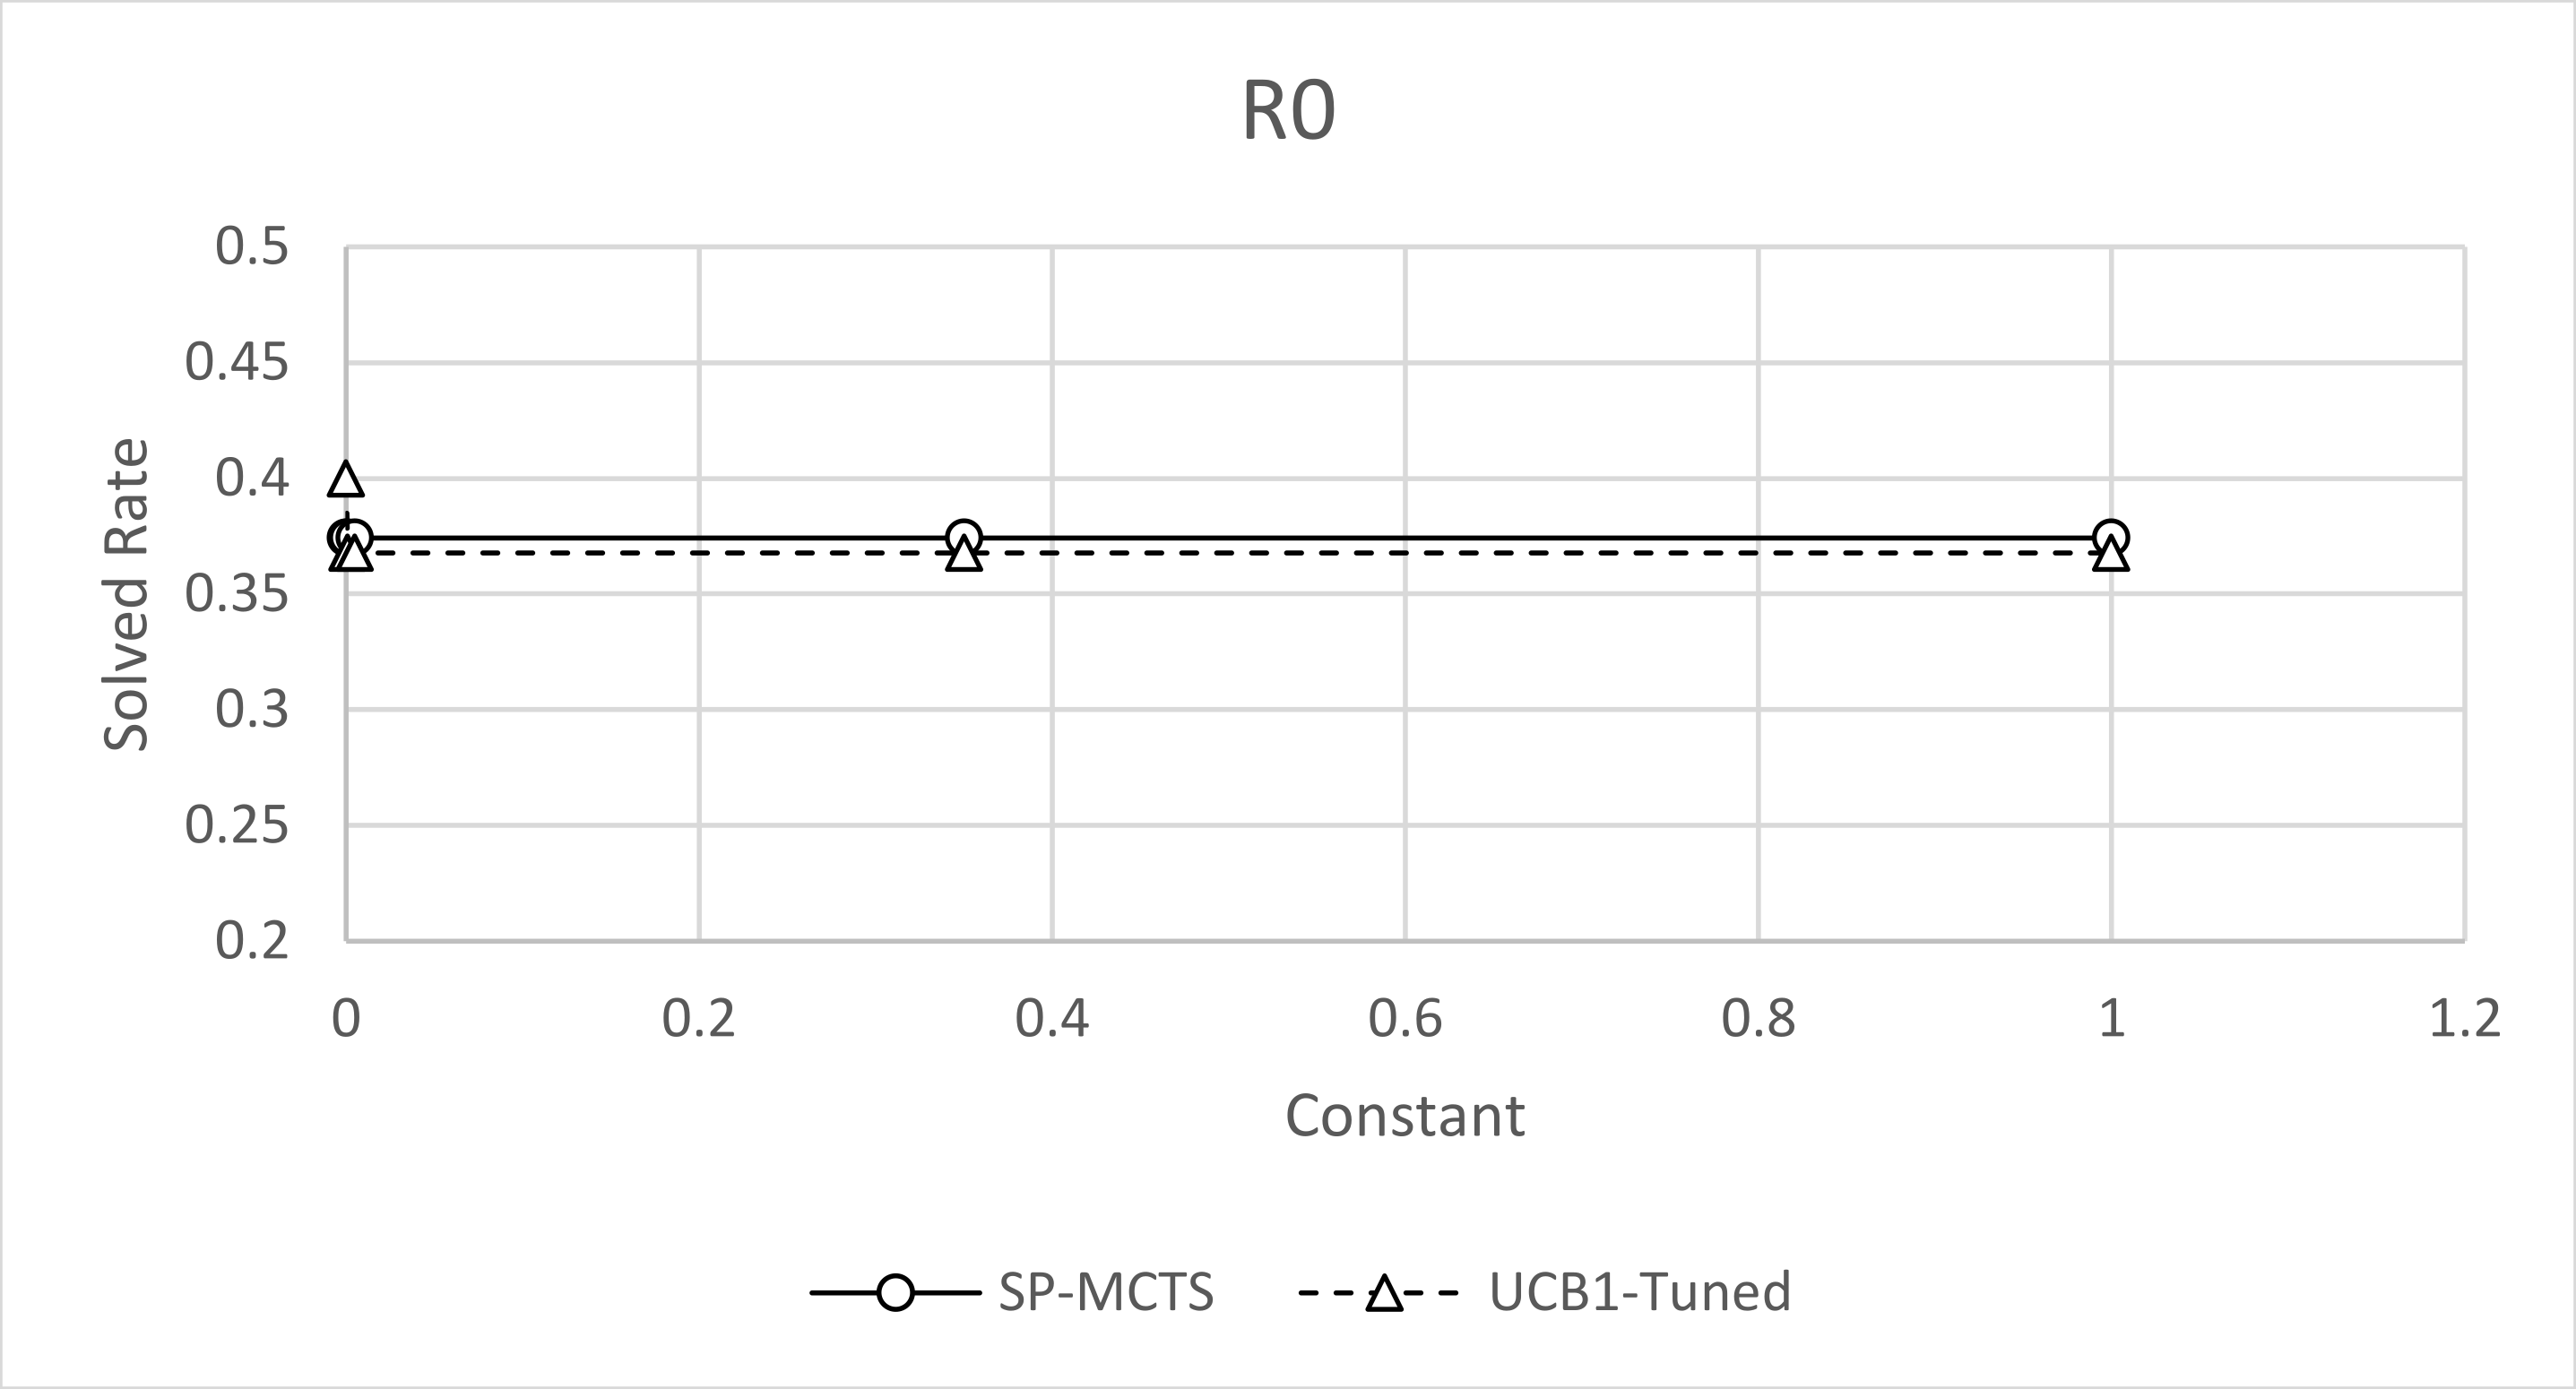
\includegraphics[width=0.8\linewidth]{pictures/Sokoban-SP-R0.png}
    \caption{SP-MCTS and UCB1-Tuned results with R0}
    \label{fig:spmcts_R0}
\end{figure}

\subsection{Node Elimination \& Cycles Avoidance}
In the following experiment we evaluated the effects of the Node Elimination and Cycles Avoidance optimizations. The baseline was obtained with standard UCT, random simulations, Node Elimination disabled and Cycles Avoidance in Stop On Cycle mode (i.e. the iteration is stopped if a cycle is detected).
\begin{figure}[!h]
    \centering
    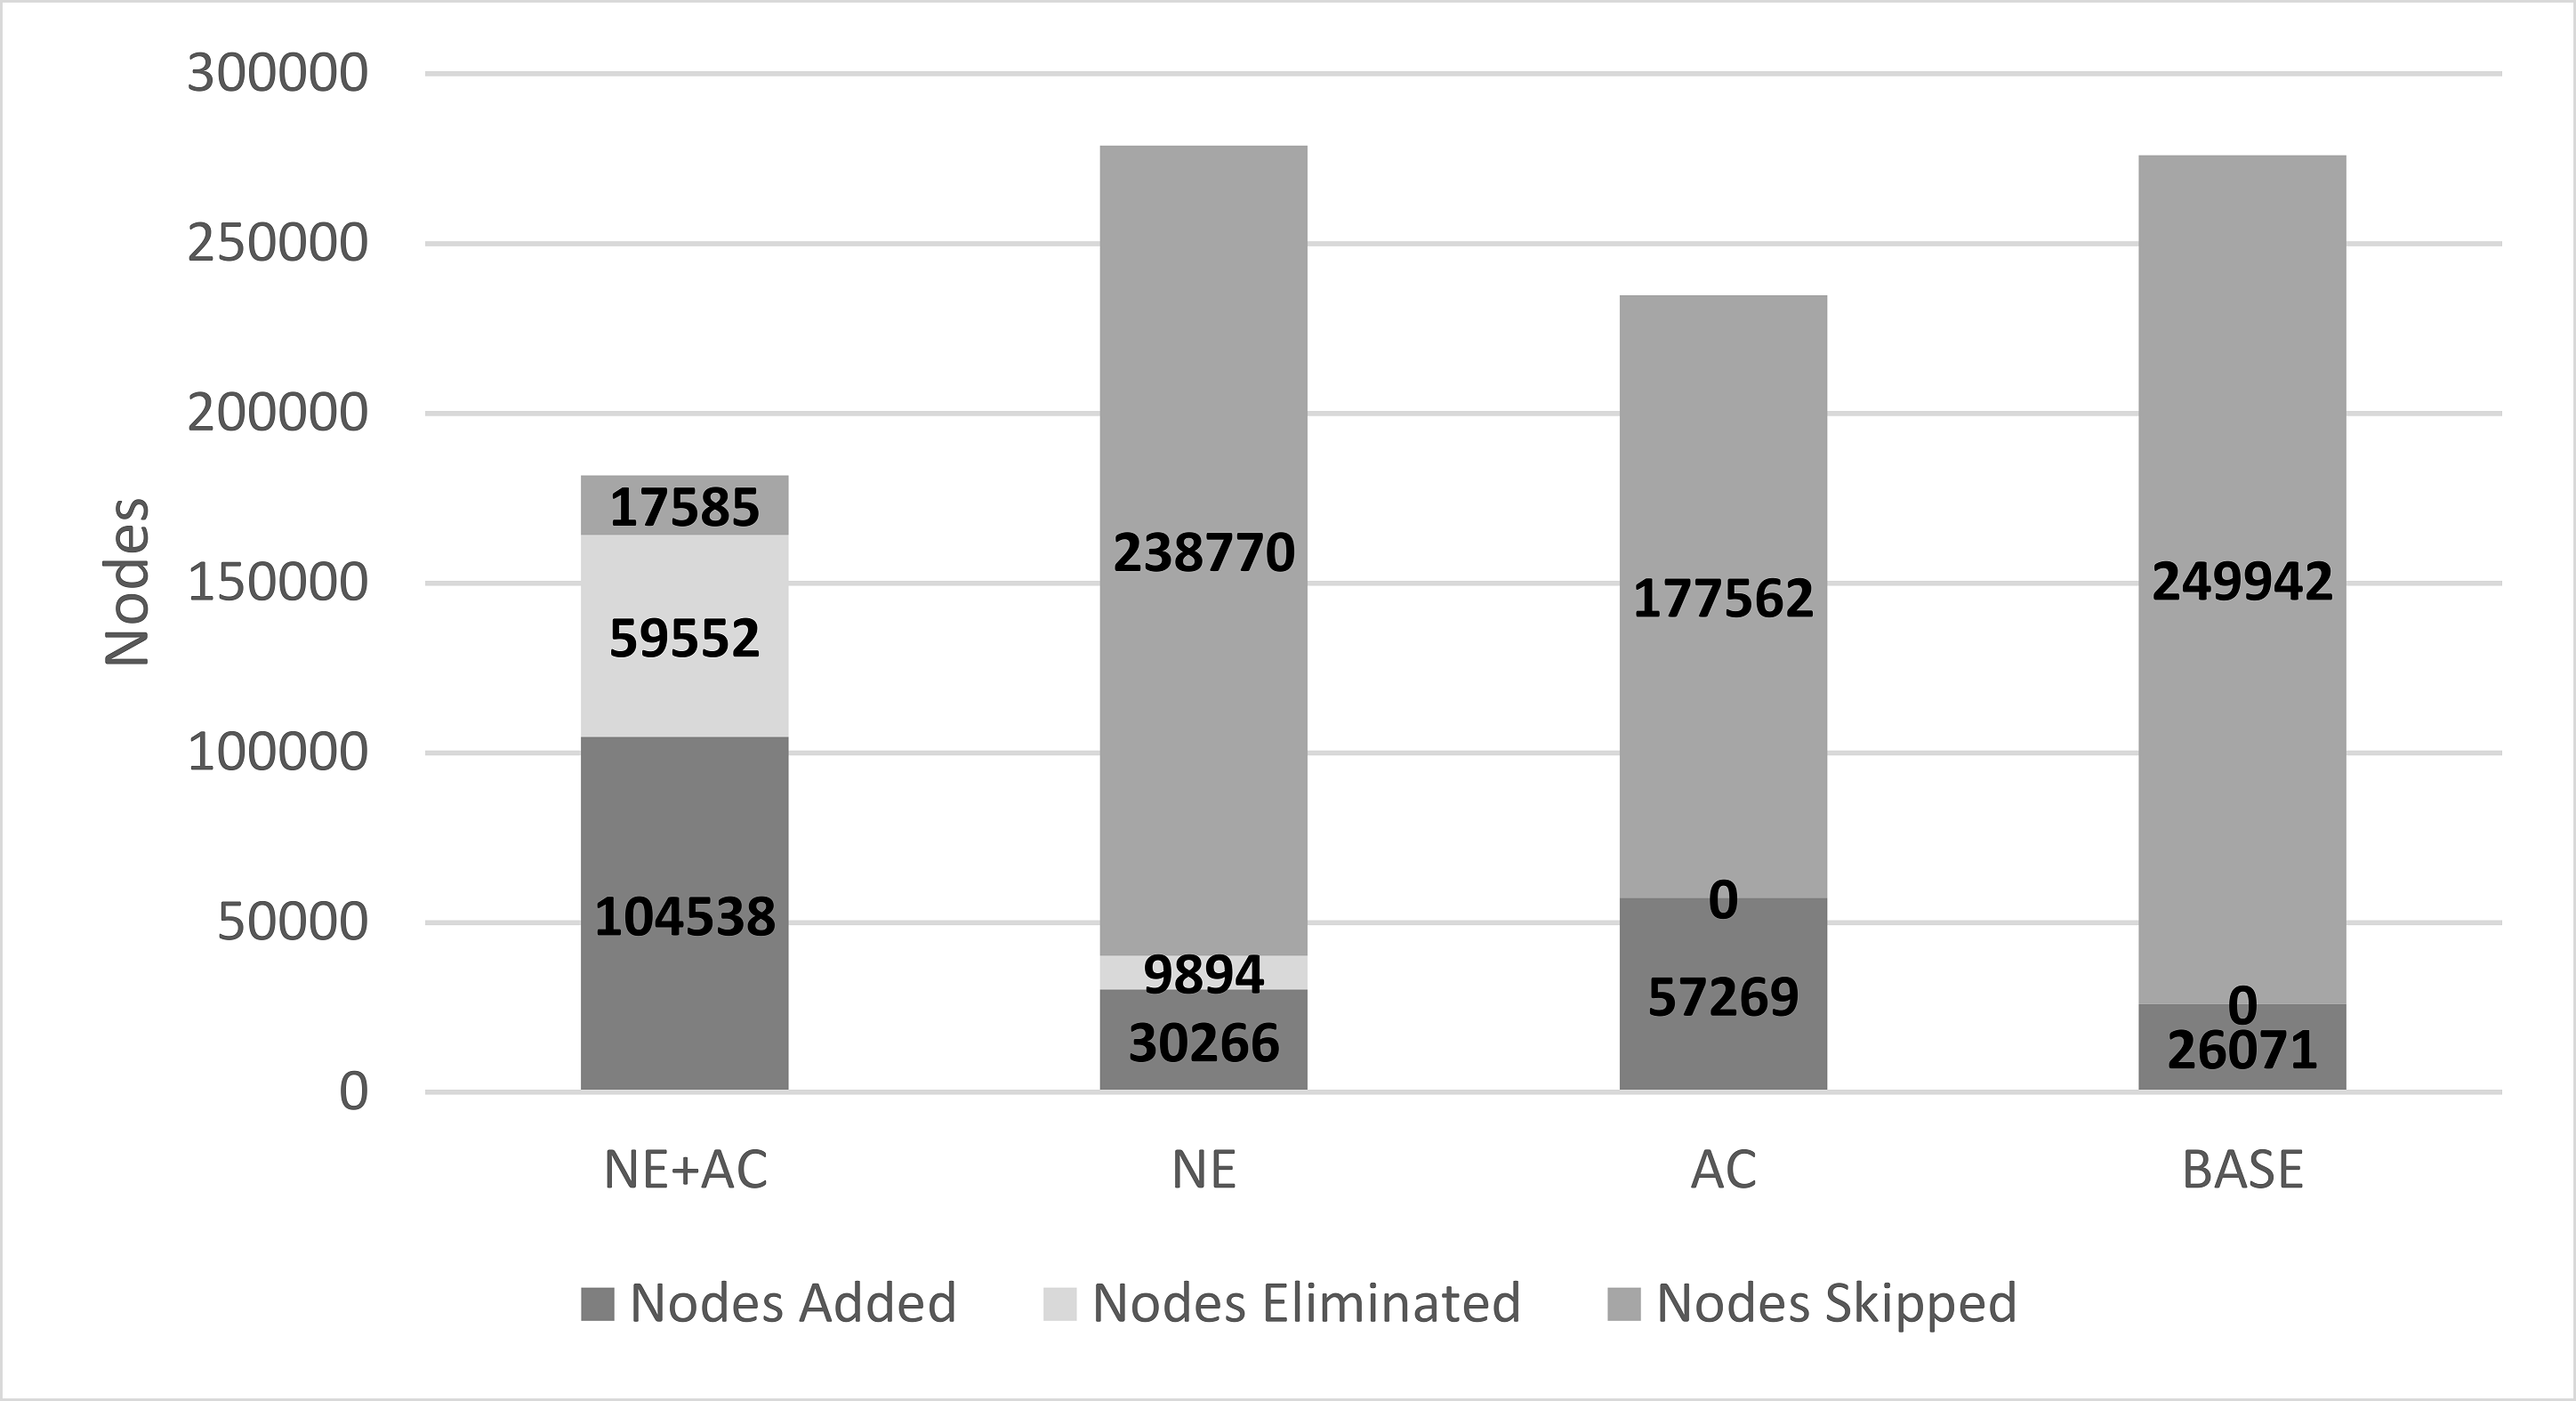
\includegraphics[width=0.9\linewidth]{pictures/SokobanNEACNodes.png}
    \caption[Node Elimination evaluation]{Nodes added, removed or skipped with combinations of Node Elimination (NE) and Avoid Cycles (AC)}
    \label{fig:SokobanNodeEliminationNodes}
\end{figure}

\medskip\noindent
Figure \ref{fig:SokobanNodeEliminationNodes} shows the number of nodes added to the search tree, the number of nodes deleted by Node Elimination and the number of iterations in which the expansion phase was skipped because the last selected node was terminal (nodes skipped). \textit{BASE} represents the baseline. We can see in Table \ref{tab:SokobanNodeEliminationNodes} how in the baseline the great majority of the iterations were executed without expanding the tree, thus terminating either on a cycle or on terminal nodes. Node Elimination prevented the algorithm from revisiting terminal nodes, causing it to slightly increase the number of nodes added to the tree, but its impact on the number of solved levels was not positive. The Avoid Cycles mode of Cycle Avoidance lead to a larger increase in the number of expanded nodes, when compared to Node Elimination. The increase in number of solved levels also lead to a decrease in the total number of iterations (as the search is stopped as soon as a solution is found). The combination of Node Elimination and Avoid Cycles obtained the best results, with far more nodes added to the tree and the highest number of solved levels.

\begin{table}[!h]
    \centering
    \begin{tabular}{l|l|l|l|l}
        Configuration & Added & Eliminated & Skipped & Solved\\
        Baseline & 9\% & 0\% & 91\% & 20\\
        Node Elimination & 11\% & 3\% & 86\% & 18\\
        Avoid Cycles & 24\% & 0\% & 76\% & 44\\
        NE + AC & 57\% & 33\%  & 10\% & 76
    \end{tabular}
    \caption[Node Elimination and Avoid Cycles evaluation]{Percentages of nodes added, eliminated and skipped, along with the number of solved levels for each configuration. The last row represents the combination of Node Elimination and Avoid Cycles}
    \label{tab:SokobanNodeEliminationNodes}
\end{table}

\medskip\noindent
Figure \ref{fig:SokobanNodeEliminationSolved} illustrates the performance of the different configurations with various number of iterations.

\begin{figure}[!h]
    \centering
    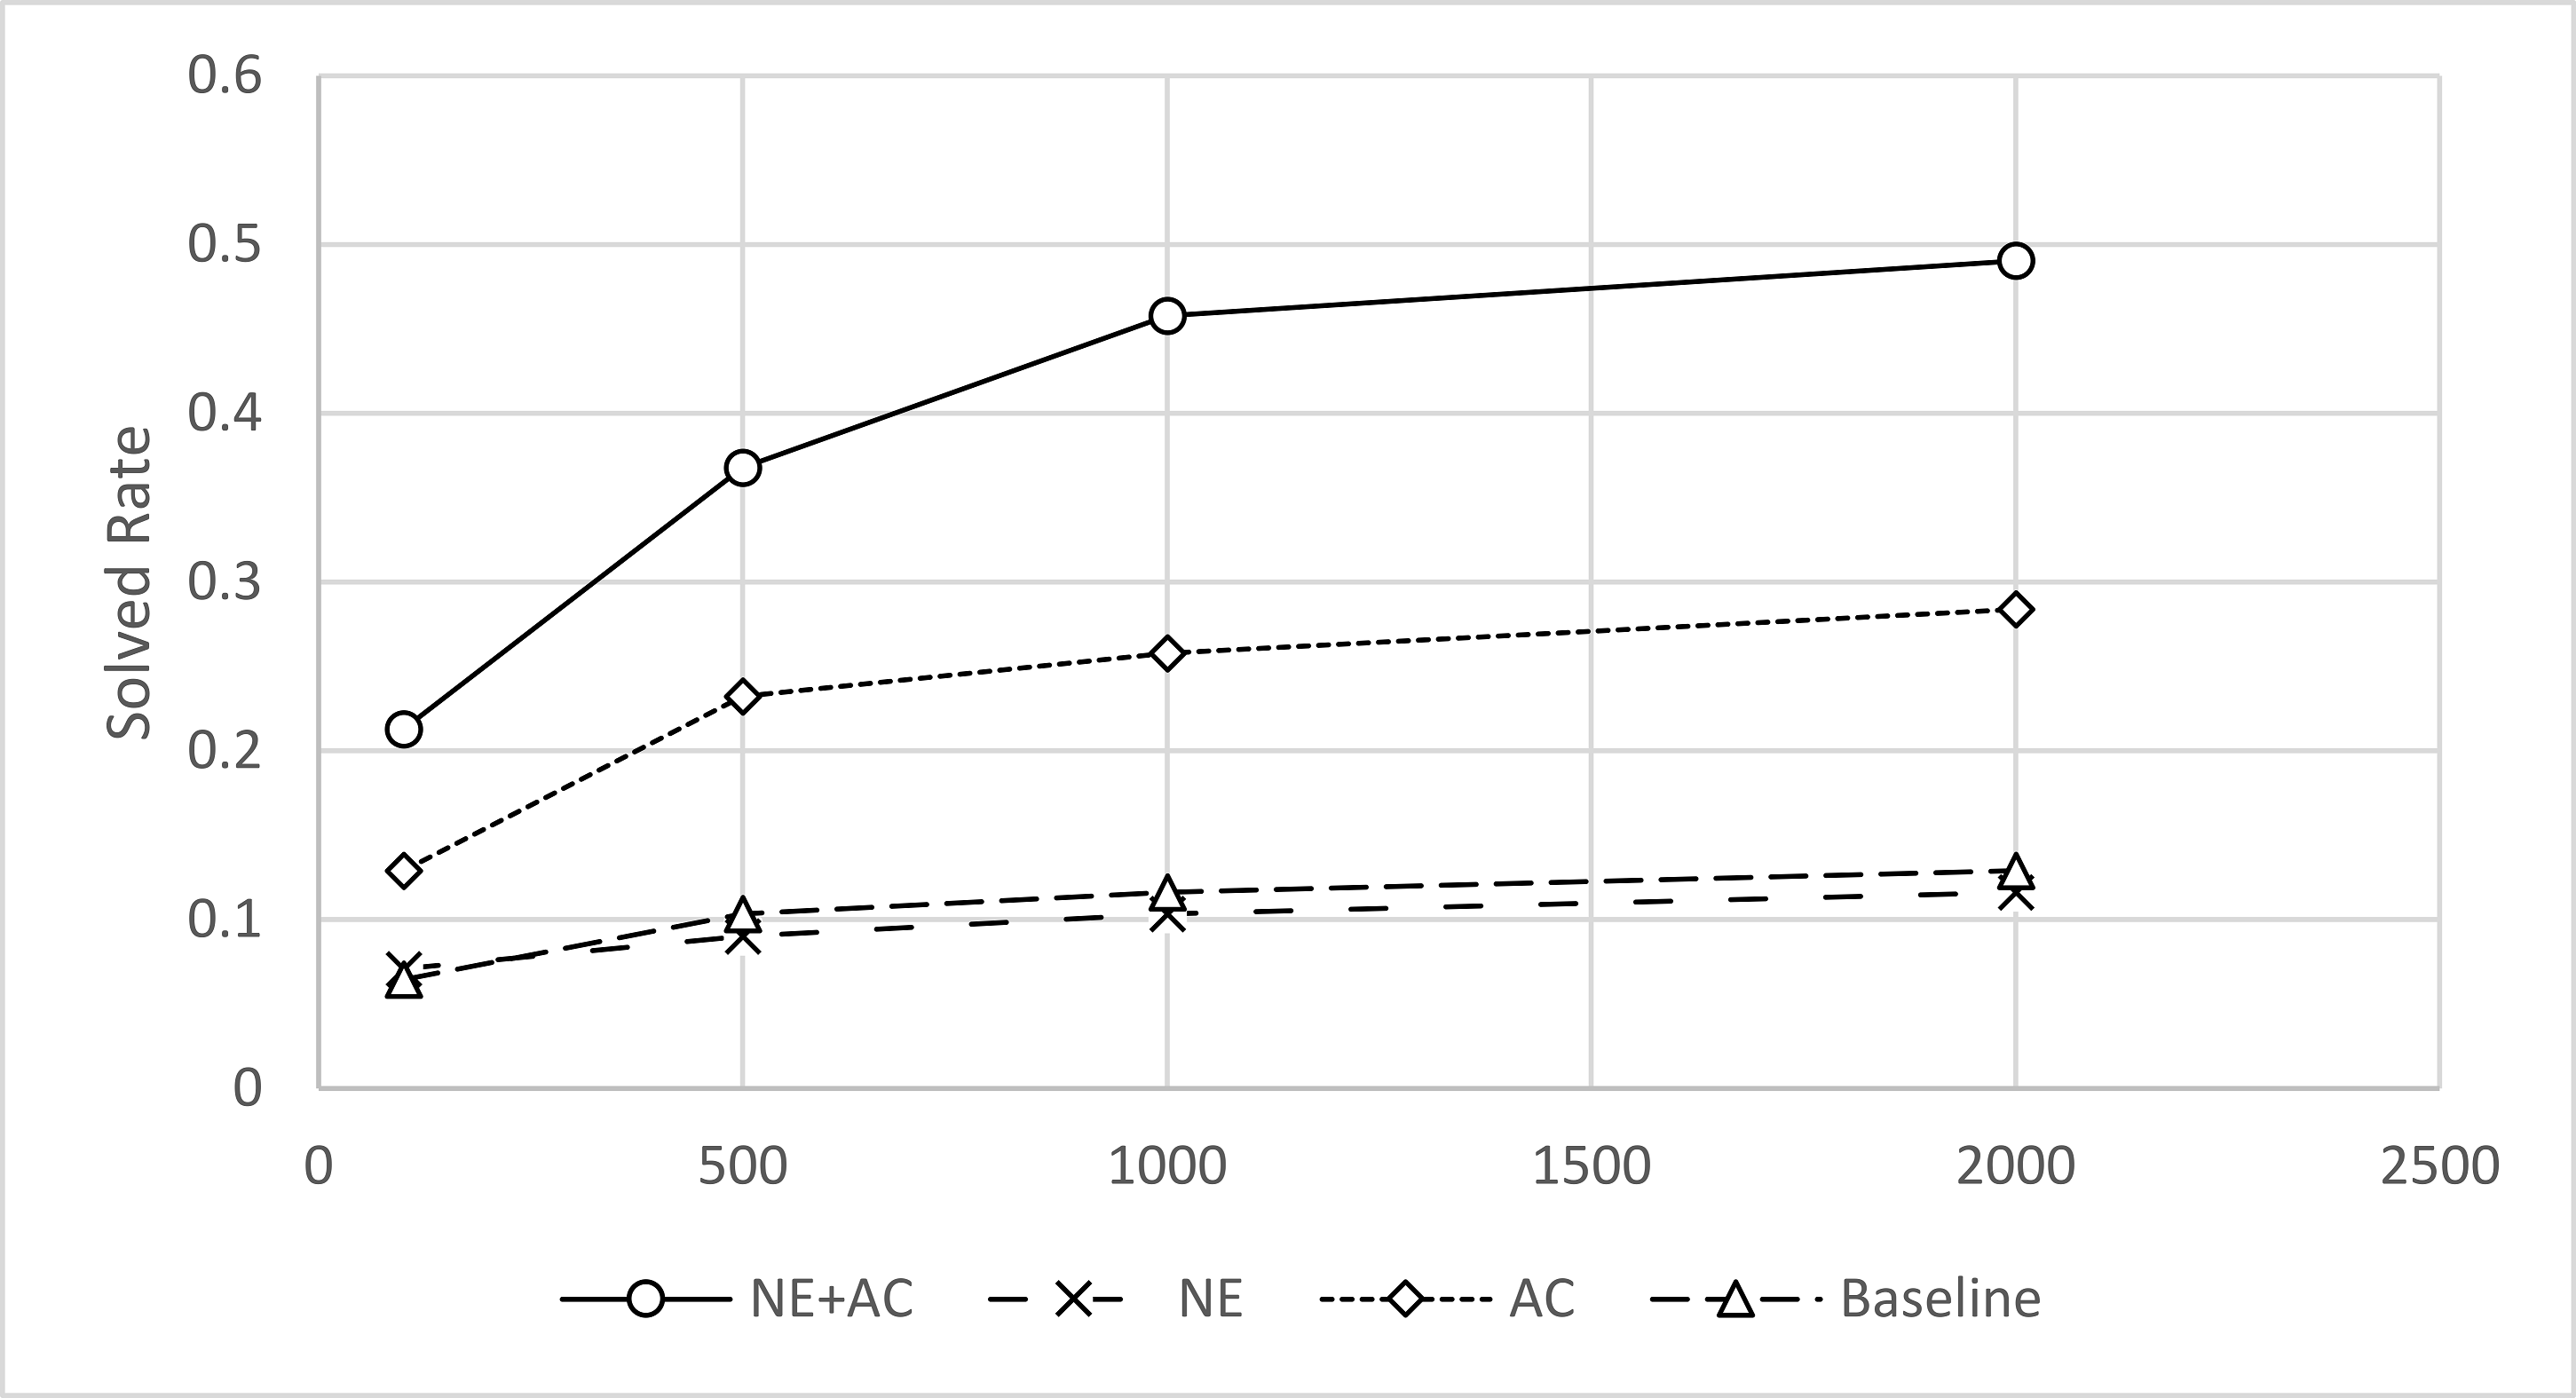
\includegraphics[width=0.9\linewidth]{pictures/SokobanNEACSolved.png}
    \caption[Node Elimination and Avoid Cycles solved levels]{Solved levels with combinations of Node Elimination (NE) and Avoid Cycles (AC) and different number of iterations}
    \label{fig:SokobanNodeEliminationSolved}
\end{figure}
\clearpage

\subsection{Parameters tuning}
\medskip\noindent
Then we tested all MCTS optimizations separately, as we done for Samegame, in order to determine the effect of each one on Sokoban and, after that, we combined all the enhancement together, trying to obtain the best result. Again we proceeded with the tuning of the parameters. In particular, we executed repeated searches with different values for the RAVE threshold and the memory budget of Node Recycling. Other enhancements such as UCB1Tuned and Node Elimination have no parameters, hence they do not require tuning.

\medskip\noindent
Table \ref{tab:sokoban_tuningrave} shows variation in term of performance on the test set as the parameter $V$ change; this parameter represents the maximum number of visits a node needs to have before the RAVE values are not used at all.

\begin{table}[!h]
    \centering
    \begin{tabular}{l|l}
        V & Solved \\
        \hline 
        1 & 45.8 \% \\
        5 & 41.9 \% \\
        10 & 42.6 \% \\
        15 & 41.9 \% \\
        25 & 42.6 \% \\
        50 & 43.8 \% \\
        100 & 42.6 \% \\
    \end{tabular}
    \caption[RAVE thresholds evaluation]{Levels solved with different RAVE thresholds. The first row is equivalent to disabling RAVE and represents our baseline.}
    \label{tab:sokoban_tuningrave}
\end{table}

\medskip\noindent
With the exception of $V=1$, which is equivalent to disabling RAVE, we can see that RAVE solved the highest number of levels with $V = 50$. However the performance was still lower than the baseline. As we did for Samegame, we concluded that the assumption necessary for RAVE to perform well does not hold for Sokoban.

\medskip\noindent
Table \ref{tab:sokoban_tuningrecycling} shows instead performance trend on the test set changing the parameter responsible for the maximum number of nodes kept in memory by the Node Recycling optimization; this parameter is used as memory budget parameter in order to keep in memory only the most promising nodes and recycling the less promising ones.
\begin{table}[!h]
    \centering
    \begin{tabular}{l|l}
        Nodes & Solved \\
        \hline 
        200 & 43.2 \% \\
        400 & 43.2 \% \\
        600 & 43.2 \% \\
        800 & 43.2 \% \\
        1000 & 45.8 \% \\
    \end{tabular}
    \caption[Node Recycling memory budgets evaluation]{Levels solved with Node Recycling and different memory budgets. The last row is equivalent to disabling Node Recycling and represents our baseline.}
    \label{tab:sokoban_tuningrecycling}
\end{table}
We can see how independently of the memory budget, Node Recycling performed uniformly worse than the baseline in Sokoban.

\subsection{Simulation policy}
\medskip\noindent
Next we tested different options for the simulation policy: we performed searches using random simulations, $\epsilon$-greedy and $\epsilon$-IDA* with different combinations of IDA* nodes and MCTS iterations. Since the IDA* simulations were significantly heavier than random and $\epsilon$-greedy ones, we compared the policies on similar execution times. The value of $\epsilon$ was set to 0.2 for both $\epsilon$-based policies. Table \ref{tab:hybridpolicies} shows the results of the various $\epsilon$-IDA* configurations. Table \ref{tab:simulationpolicies} shows the comparison between $\epsilon$-IDA*, $\epsilon$-greedy and random simulation policies. $\epsilon$-greedy solved 95 levels

\begin{table}[!h]
    \centering
    \begin{tabular}{ l | l | l | l }
        IDA* Nodes & MCTS Iterations & Time & Solved \\
        \hline
        100 & 100 & 1h 13m 21s & 55.5\% \\
        20 & 500 & 1h 28m 30s & 54.2\% \\
        5 & 1000 & 1h 0m 50s & 54.2\% \\
    \end{tabular}
    \caption[Results of $\epsilon$-IDA*]{Results of $\epsilon$-IDA*. Each row represents one configuration.}
    \label{tab:hybridpolicies}
\end{table}


\begin{table}[!h]
    \centering
    \begin{tabular}{l|l|l|l}
        Policy & Iterations & Time & Solved \\
        \hline
        $\epsilon$-IDA*(100) & 100 & 1h 13m 21s & 55.5\%\\
        $\epsilon$-greedy & 5000 & 1h 9m 47s & 61.3\% \\
        Random & 5000 & 1h 11m 55s & 52.3\% \\
    \end{tabular}
    \caption{Results of the different simulation policies.}
    \label{tab:simulationpolicies}
\end{table}

\subsection{Sokoban complexity}
During our experiments we noticed that contrary to what we expected, the performance of MCTS didn't improve much when increasing the number of iterations. When comparing the number of levels solved relative to the number of nodes used in IDA* and the number of iterations performed in MCTS, we noticed a similar trend (Figures \ref{fig:sokobanIDAComplexity} and \ref{fig:sokobanMCTSComplexity}). After reaching a certain threshold, the resources needed to solve additional levels increase dramatically. We consider this to be a consequence of the quality of the heuristic evaluation which is not suitable for levels in which boxes must be pushed away from goals in order to find a solution. It's still not clear why the threshold in MCTS appears earlier than in IDA*.

\begin{figure}[!h]
    \centering
    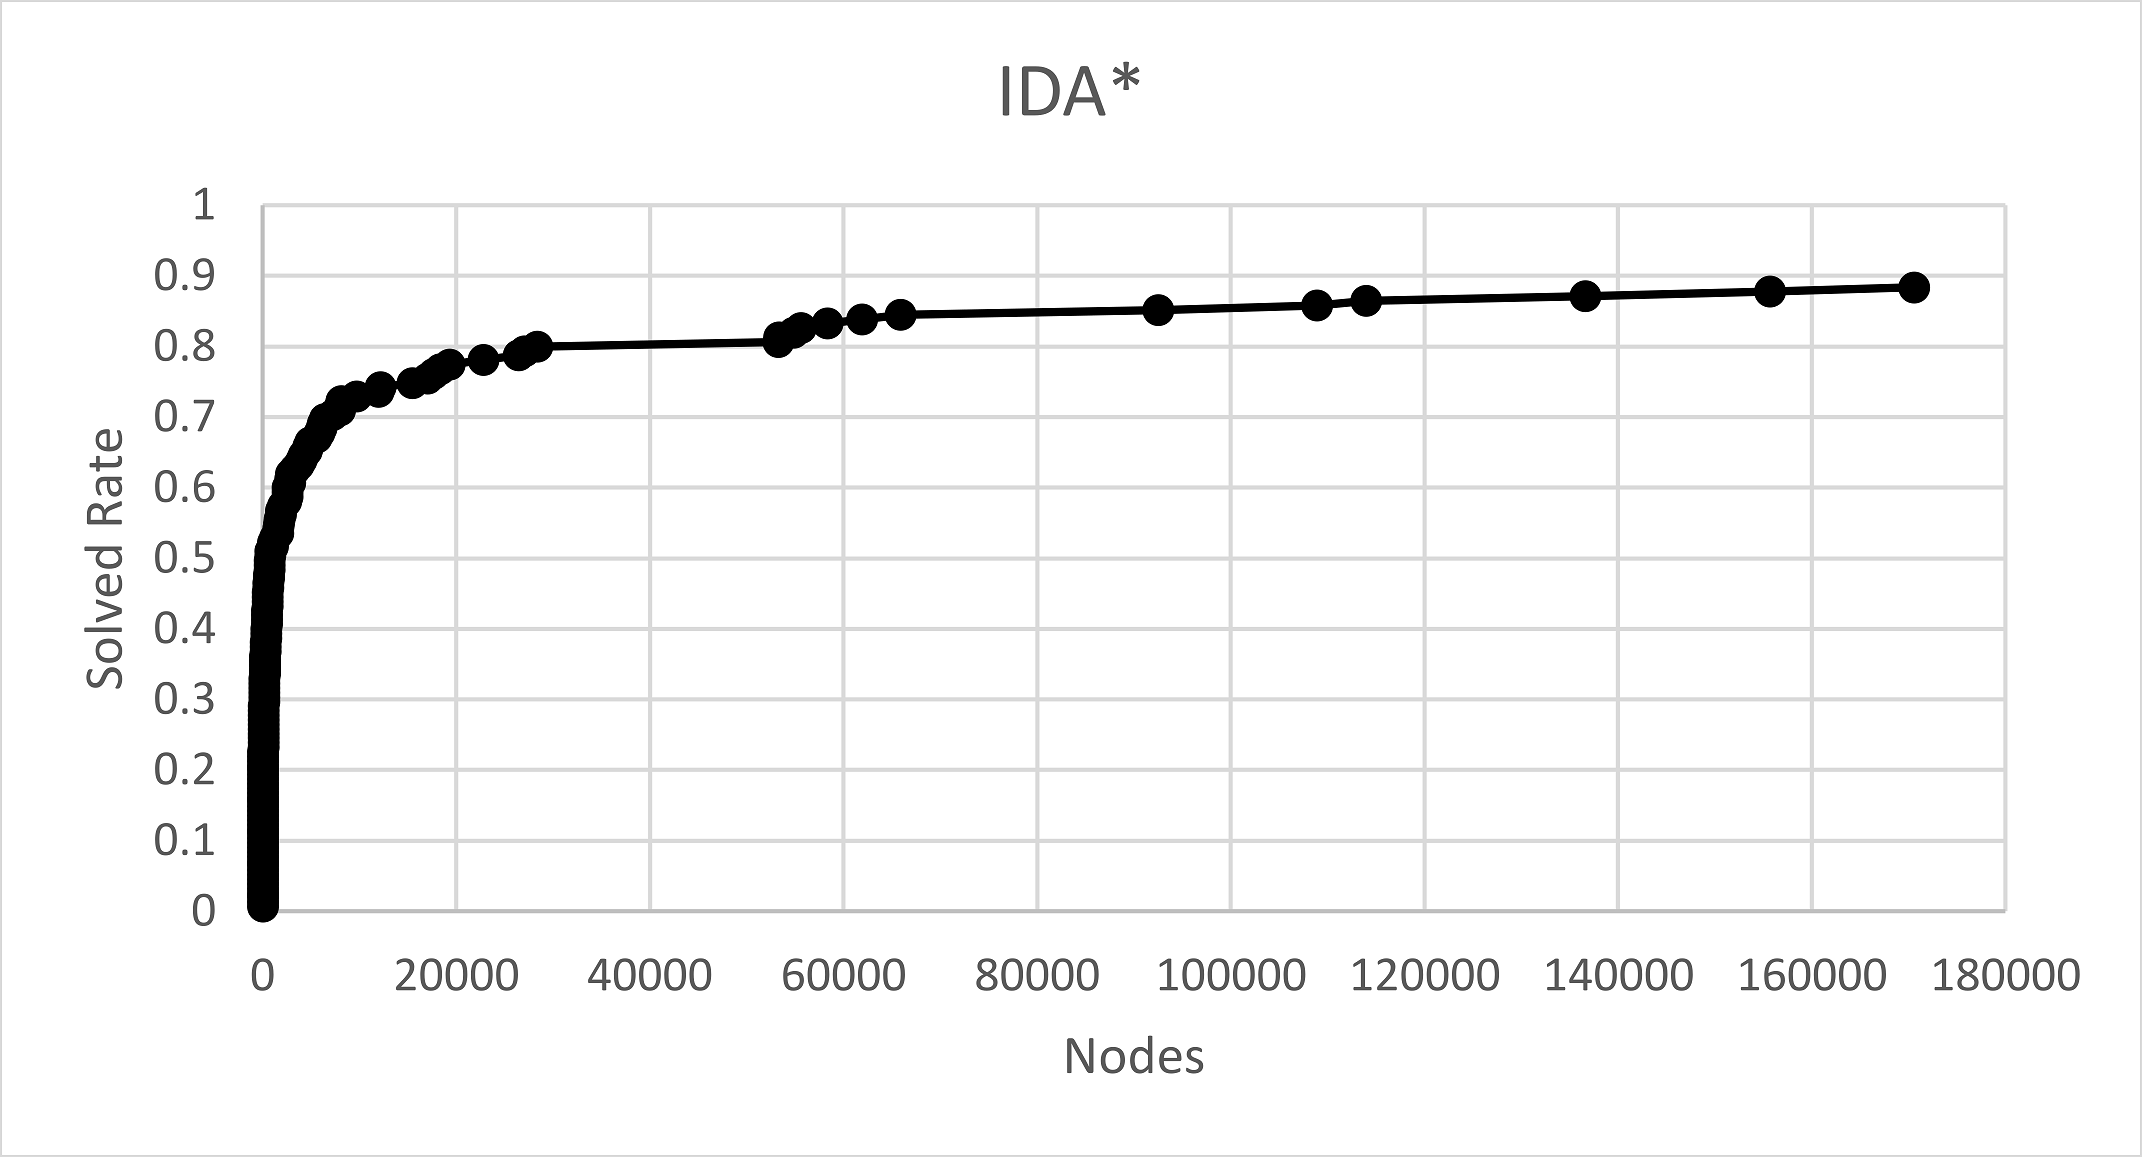
\includegraphics[width=0.8\linewidth]{pictures/SokobanIDAComplexity.png}
    \caption[IDA* solved levels]{Levels solved according to number of nodes used in IDA*}
    \label{fig:sokobanIDAComplexity}
\end{figure}
\clearpage

\begin{figure}[!h]
    \centering
    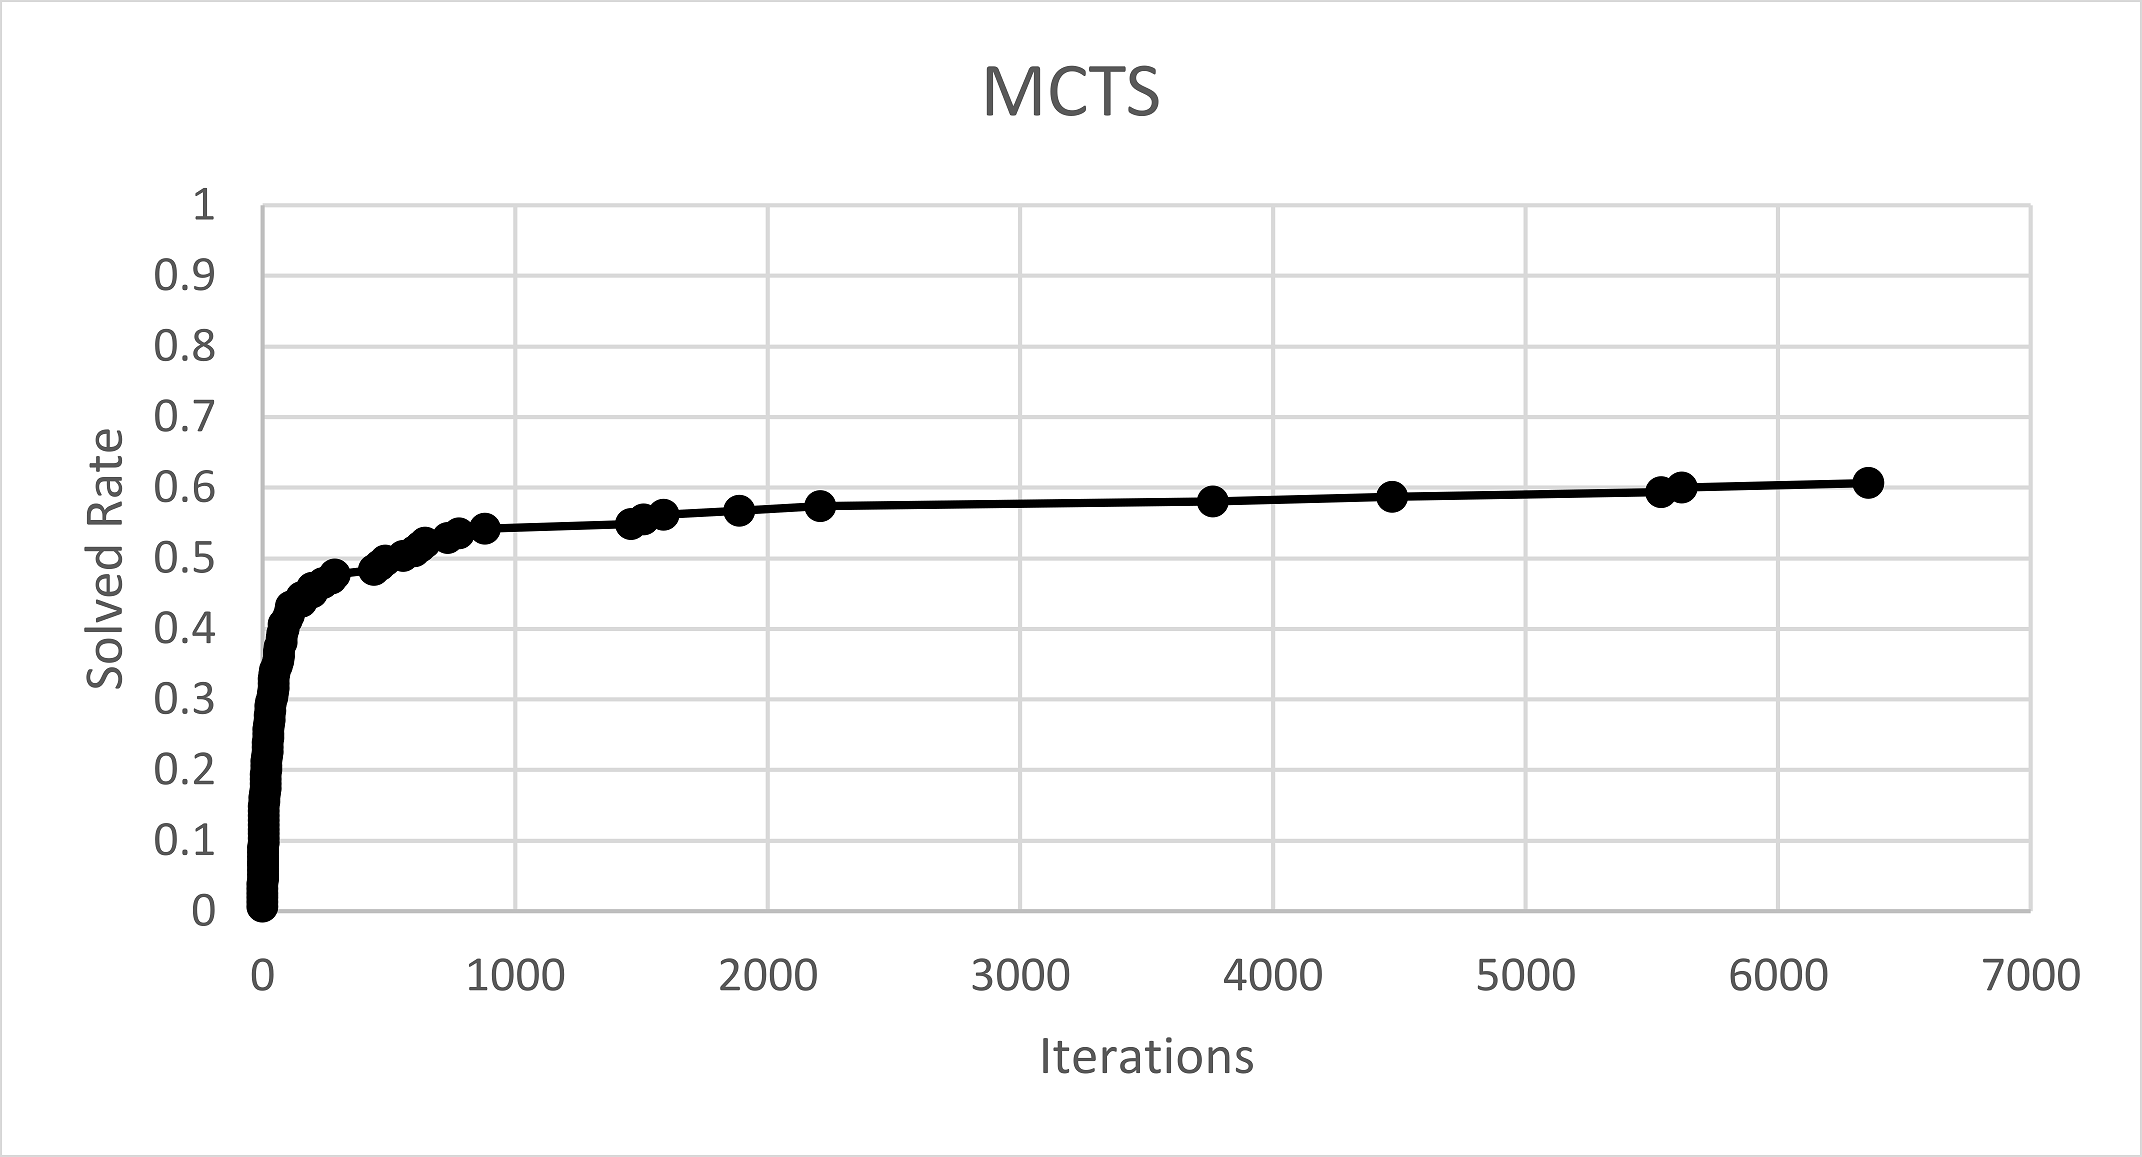
\includegraphics[width=0.8\linewidth]{pictures/SokobanMCTSComplexity.png}
    \caption[MCTS solved levels]{Levels solved according to number of iterations performed in MCTS}
    \label{fig:sokobanMCTSComplexity}
\end{figure}

\subsection{Results}
The last experiment we performed consisted in the comparison between IDA* and different versions of MCTS for Sokoban. For this final comparison we used three versions of MCTS based on the formula used for the estimation of the action-value function: standard UCT, UCB1-Tuned and SP-MCTS. Standard MCTS used NegativeBM as a reward with a constant of 6. UCB1-Tuned used InverseBM as a reward with a constant of 0.05. SP-MCTS used NegativeBM as a reward, with a constant of 2. Node Elimination and Cycles Avoidance were enabled in all three configurations. To keep a comparable search time between all methods, IDA* used a maximum of 200000 nodes and all MCTS methods used 10000 iterations with $\epsilon$-greedy as a simulation policy, with $\epsilon=0.2$. Table \ref{tab:sokoban_results} shows the final results of this comparison.
\begin{table}[!h]
    \centering
    \begin{tabular}{l|l}
        Method & Solved \\
        \hline
        IDA* & 88.4\%\\ 
        UCT & 64.5\%\\
        UCB1-Tuned & 54.8\%\\
        SP-MCTS & 60.6\%\\
    \end{tabular}
    \caption{Methods comparison}
    \label{tab:sokoban_results}
\end{table}
\clearpage
\medskip\noindent
IDA* solved the highest number of levels with respect to the other methods. Among MCTS methods, UCT achieved the best performance with 64.5\% of solved levels.